\documentclass[12pt,openany,twoside,letterpaper]{book}

%Muestra los márgenes del documento para evitar Warnings
%Para activar la siguiente línea quite el simbolo % 
%\usepackage[showframe]{geometry}

%Usando el paquete BibLaTeX
%Cita normal con \cite[página]{} y cita con paréntesis \parencite[página]{}

% Configuración de BibLaTeX
%\usepackage[backend=biber,style=authoryear,maxcitenames=2,maxbibnames=99,giveninits=true,uniquename=false]{biblatex}
%\addbibresource{biblio.bib}

% Personalizar el formato de las citas y la bibliografía
%\DeclareNameAlias{sortname}{family-given}
%\DeclareDelimFormat{multinamedelim}{\addcomma\space}
%\DeclareDelimFormat{finalnamedelim}{\addcomma\space\&\space}
%\DeclareFieldFormat{titlecase}{\MakeSentenceCase*{#1}}
%\DeclareFieldFormat[article,inbook,incollection,inproceedings,patent,thesis,unpublished]{title}{\titlecase{#1}}
%\DeclareFieldFormat{journaltitlecase}{\titlecase{#1}}
%\DeclareFieldFormat{pages}{#1}
%\DeclareFieldFormat{volume}{\mkbibbold{#1}}
%\renewbibmacro{in:}{}
%\AtEveryBibitem{\clearfield{month}}

\usepackage[spanish]{babel}
\usepackage[utf8]{inputenc}
% Carácteres especiales
\usepackage{fontenc}
% More advance packages


\usepackage[utf8]{inputenc}
\usepackage[T1]{fontenc}
\usepackage{forest}
\usetikzlibrary{decorations.pathreplacing, calc, positioning}

% Configuration for the "Brace" decoration
\tikzset{
    description/.style={
        text width=5cm,
        align=left,
        font=\footnotesize\sffamily,
        anchor=west,
        xshift=0.2cm
    },
    mybrace/.style={
        decorate,
        decoration={brace, amplitude=5pt, mirror}, % Mirror makes it face right
        thick,
        draw=black
    }
}


\usepackage{tikz}
\usetikzlibrary{shapes, arrows.meta, positioning, chains, fit, backgrounds, patterns, babel, shadows}
\usepackage{xcolor}


\usepackage{amssymb,amsbsy,mathrsfs,rotating,float,multirow,upgreek,amsmath,lineno,bm}
\usepackage{breakcites}
\usepackage{listings}
\usepackage{pgfplots}
\pgfplotsset{compat=1.18}

\usepgfplotslibrary{groupplots}
\usepackage{longtable}
\setlength{\LTcapwidth}{6in}
\usepackage[utf8]{inputenc}
\usepackage{epsfig,epic,eepic,threeparttable,amscd,here,lscape,tabularx,graphicx }
\usepackage{booktabs}
\usepackage{array}
\usepackage{overpic}
\usepackage{microtype}
%%%%%%%%%%%
%\usepackage{newtxtext,newtxmath}
%%%%%%%%%%%
%\usepackage[table]{xcolor}
\usepackage{caption}
\usepackage{subcaption}
% Permite ver y configurar los parámetros de la página
\usepackage{layout}
%Hyperref permite ver las secciones del texto
\usepackage[hidelinks]{hyperref}
\usepackage{cleveref}
\usepackage{lmodern}
\usepackage{nomencl}
\usepackage[T1]{fontenc}
%% This code creates the groups
% -----------------------------------------
\renewcommand{\nomname}{\sffamily List of Symbols and Abbreviations} 

\usepackage{etoolbox}
\renewcommand\nomgroup[1]{%
  \item[\Large\bfseries
  \ifstrequal{#1}{A}{Number Sets}{%
  \ifstrequal{#1}{B}{Symbols}{%
  \ifstrequal{#1}{C}{Abbreviations}{}}}%
]\vspace{10pt}}
\makenomenclature
% -----------------------------------------

\newcommand{\todo}[1]{\textcolor[rgb]{1.00,0.00,0.00}{#1}}




\providecommand{\var}[1]{{\ensuremath{var}}\{#1\}}
\DeclareMathOperator{\tire}{\negthinspace-\negthinspace}
\DeclareRobustCommand{\legend}[1]{%
	\textcolor{#1}{\rule{1ex}{2ex}}%
}
\newcommand{\lineplot}[1]{
	\textcolor{#1}{\rule{1.5ex}{0.3ex}}%
}

%%%% custom colors
\colorlet{color0}{blue!40!gray}% pearson *
\colorlet{color1}{blue!80!gray} %pearson **
\colorlet{color2}{red!40!gray} %n-pearson*
\colorlet{color3}{red!80!gray}%n-pearson**
\colorlet{color4}{green!40!gray} %plv*
\colorlet{color5}{green!80!gray} 

\definecolor{frontal}{RGB}{141, 211, 199}
\definecolor{frontal_left}{RGB}{255, 237, 111}
\definecolor{frontal_right}{RGB}{255, 255, 179}
\definecolor{central_right}{RGB}{251, 128, 114}
\definecolor{central_left}{RGB}{204, 235, 197}
\definecolor{posterior_right}{RGB}{253, 180, 98}
\definecolor{posterior_left}{RGB}{217, 217, 217}
\definecolor{posterior}{RGB}{179, 222, 105}


%%%%
\definecolor{darkorange25512714}{RGB}{255,127,14}
\definecolor{forestgreen4416044}{RGB}{44,160,44}
\definecolor{steelblue31119180}{RGB}{31,119,180}

% Colors for state_of_art.tex mindmap
\definecolor{softblue}{RGB}{100, 149, 237}
\definecolor{hardred}{RGB}{205, 92, 92}
\definecolor{predgreen}{RGB}{60, 179, 113}
%%%%

\newcommand{\Objectiveonename}{}
\newcommand{\Objectivetwoname}{}
\newcommand{\Objectivethreename}{}

%% defining objective names
% \renewcommand{\Objectiveonename}{Develop a neural networks-based optimization strategy that is adaptable to different noise levels and specific restrictions, ensuring results comparable to conventional optimization techniques in terms of compliance with resSingle-trial kernel-based functional connectivity for enhanced feature extriactions and robustness in EEG-based MI-BCI}
% \renewcommand{\Objectivetwoname}{
% Develop a customized neural networks-based non-linear programming optimization scheme for gas-powered energy systems that considers physical limits and non-differentiable functions, focusing on modeling gas supply behavior and compliance with system constraintsKCS-FCnet: Kernel Cross-Spectral Functional Connectivity Network for automatic EEG representation in MI-BCI}
% \renewcommand{\Objectivethreename}{Develop a customized neural networks-based non-linear programming optimization strategy for the Colombian gas-powered energy system, modeling the behavior of supply-demand flows and pressures and incorporating physical boundaries and non-differentiable functions that ensure efficiency over time and convergencequalitative and quantitative post-hoc and intrinsic interpretation for MI-BCI models}

%%%


% Create author commands
\newcommand{\studentname}{}
\newcommand{\submissiondate}{}
\newcommand{\academictitle}{}
\newcommand{\resgroupone}{}
%\newcommand{\resgrouptwo}{}
\newcommand{\researchtopic}{}
\newcommand{\thesisname}{}
\newcommand{\thesisnamespanish}{}
\newcommand{\director}{}
\newcommand{\codirector}{}
\newcommand{\issuedate}{}
\newcommand{\palabrasclave}{}
\newcommand{\keywords}{}
\newcommand{\schlusselworter}{}
\newcommand{\palavraschave}{}
\newcommand{\sede}{}
\newcommand{\department}{}
\newcommand{\faculty}{}

%Información de la tesis
%Diligenciar aquí los datos para su carga automática donde se requiera en el documento
\renewcommand{\studentname}{Julian Andres Salazar Parias}
\renewcommand{\thesisname}{An Embedded Framework for EEG-Based Neurophysiological Data Acquisition to Support ADHD Monitoring}
\renewcommand{\thesisnamespanish}{Marco Integrado para la Adquisición de Datos Neurofisiológicos Basados en EEG para Apoyar la Monitorización del TDAH}
\renewcommand{\issuedate}{2025}
\renewcommand{\submissiondate}{2025}
\renewcommand{\director}{M.Sc. Bernardo Andrés Cardona Noreña}
\renewcommand{\codirector}{Ph.D. Andrés Marino Álvarez Meza}
\renewcommand{\academictitle}{Maestría en ingeniería - Automatización Industrial}
\renewcommand{\resgroupone}{Grupo de Control y Procesamiento Digital de Señales (GCPDS) }
%\renewcommand{\resgrouptwo}{}
\renewcommand{\researchtopic}{Inteligencia Artificial}
\renewcommand{\sede}{Manizales} 
\renewcommand{\department}{Departamento de ingeniera eléctrica, electrónica y computación}
\renewcommand{\faculty}{Facultad de ingeniera y arquitectura}


%Palabras clave del documento - Tener presente los Theasurus https://www.thesaurus.com/
%Disponible en 3 idiomas aunque se puede extender a francés o otro idioma

\renewcommand{\palabrasclave}{Use palabras clave que estén en Theasaurus} 
\renewcommand{\keywords}{Use keywords available in Theasaurus}

% Estilo de los encabezados y pies de página
\usepackage{fancyhdr}

\fancyhf{}%
\pagestyle{fancyplain}
\textheight22.5cm \topmargin0cm \textwidth16.5cm \headheight25.33461pt
\oddsidemargin0.5cm \evensidemargin-0.5cm%
\fancypagestyle{plain}{
\fancyhead[RO,LE]{}
\fancyhead[RE,LO]{\small \textbf{\thesisname}}
\fancyfoot[CO,CE]{\thepage}
}
\pagestyle{fancy}
\fancyhf{}% Clear all header and footer fields
\renewcommand{\chaptermark}[1]{\markboth{\thechapter.\; #1}{}}
% \renewcommand{\sectionmark}[1]{\markright{\thesection.\; #1}{}} % Comentado para no usar secciones en encabezados
\fancyhead[LO,RE]{\leftmark} % Pone el nombre del capítulo en el encabezado izquierdo de las páginas impares y en el derecho de las páginas pares
% \fancyhead[RO,LE]{\rightmark} % Comentado para no poner nombre de sección en el encabezado
\fancyfoot[CO,CE]{\thepage} % Pone el número de página en el centro del pie de página
\thispagestyle{fancy}% Ensure that the first page of each chapter will have headers and footers as well



\usepackage{titlesec}
% Permite personalizar los títulos de sección y de capítulos
% hang lo deja en el mismo renglón, display lo despliega
% Elimina el "Capitulo" y deja solo el número

\titleformat{\chapter}[hang]
  {\sffamily\Huge\bfseries}{\thechapter}{0.5cm}{\sffamily\Huge}
\titleformat{\section}[hang]{\sffamily\LARGE}{\thesection}{0.5cm}{}
\titleformat{\subsection}[hang]{\sffamily\Large}{\thesubsection}{0.5cm}{}
\titleformat{\subsubsection}[hang]{\sffamily\large}{\thesubsubsection}{0.5cm}{}
\titleformat{\paragraph}[runin]{\sffamily\normalsize}{}{}{\emph}

%Coloca anexo o apéndice en la Tabla de contenido
\usepackage[toc,page]{appendix}

% Configuración de las páginas en twoside-mode
% Permite ver y configurar los parámetros de la página
\setlength{\voffset}{-0.25in}
\setlength{\headwidth}{467pt}
\setlength{\headheight}{25.33461pt}
\setlength{\oddsidemargin}{0pt}
\setlength{\evensidemargin}{0pt}
\setlength{\marginparwidth}{0pt}
\setlength{\marginparsep}{0pt}
\setlength{\parskip}{2em}
\setlength{\footskip}{20pt}
\setlength{\textheight}{650pt}
\setlength{\textwidth}{467pt}
\setlength{\headsep}{5pt}
\setlength{\parindent}{0pt}
\setlength{\baselineskip}{10pt plus 5pt minus 5pt}
\renewcommand{\theequation}{\thechapter-\arabic{equation}}
\renewcommand{\thefigure}{\textbf{\thechapter-\arabic{figure}}}
\renewcommand{\thetable}{\textbf{\thechapter-\arabic{table}}}

%Define la distancia de la primera linea de un parrafo a la margen
\parindent0cm 

%Espacio entre lineas
\renewcommand{\baselinestretch}{1}

%Para rotar texto, objetos y tablas seite.
\usepackage{rotating}


%Permite incluir mecanismos y reacciones químicas
\usetikzlibrary{positioning}
\usetikzlibrary{mindmap}
\usepackage{chemformula}
\usepackage{chemfig}
\usepackage{xcolor}

\usetikzlibrary{calc,arrows.meta}% per right to e left to
\tikzset{
myedge/.style={->, -{Latex[#1]}}
}

%Fuente de la presentación Ancizar Sans UNAL
%Para usar este compilado en Overleaf se debe usar el compilador XeLaTeX o LuaLaTeX!!
%Menu -> Compiler -> XeLaTeX o LuaLaTeX
%La siguiente línea debe comentarse si desea compilar con pdfLaTeX
%\RequireXeTeX

% Definición de la fuente Ancizar Sans
\newif\ifxetexorluatex

\ifxetexorluatex
  \usepackage{fontspec}
  \usefonttheme{serif}
  \setmainfont{AncizarSans}[Path=./AncizarSans/,Scale=1,Extension=.otf,UprightFont=*-Regular,BoldFont=*-Bold,ItalicFont=*-Italic,BoldItalicFont=*-BoldItalic]
\else
  % Si se compila con pdfLaTeX, cargar la fuente apropiada aquí
  \usepackage[T1]{fontenc}
\fi
% Metadatos del documento
\AtBeginDocument{%
	\hypersetup{
		pdfborder={0 0 0},
		pdfauthor={\studentname},
		pdfsubject={\thesisname}, 
		pdfcreator={\studentname},
		pdfproducer={\studentname},
	}
}

%Carga el simbolo de grado y el de Angstrom
\newcommand{\angstrom}{\textup{\AA}}
\newcommand{\grad}{$^{\circ}$}

\newtheorem{theorem}{Theorem}
\newtheorem{lemm}[theorem]{Lemma}
\newtheorem{proof}{Proof}[theorem]
\newtheorem{propo}[theorem]{Proposition}

\usepackage[acronym=true, 
            toc=true, 
            numberline=false, 
            nopostdot=true, 
            section=chapter, 
            nomain=true]{glossaries-extra}
\setabbreviationstyle[acronym]{long-short}
\renewcommand{\glsnamefont}[1]{\textsc{\normalfont\large #1}}
\glssetcategoryattribute{acronym}{hyperoutside}{false}
%Inicio del documento, no olvide la etiqueta de cierre al final \end{document}
%\newglossary*{symbols}{List of Symbols}
\newglossary[slg]{symbols}{not}{ntn}{Symbols}


\newglossaryentry{ip}
{
    name={IP},
    description={Inner Point},
    type=acronym,
    sort={ip}
}
\newglossaryentry{pi}
{
    name={\ensuremath{\pi}},
    description={ratio of circumference of circle to its
            diameter},
    type=symbols,
    sort={pi}
}
\newglossaryentry{upme}
{
    name={UPME},
    description={Unidad de Planeación Minero Energética},
    type=acronym,
    sort={upme}
}

\newglossaryentry{creg}
{
    name={CREG},
    description={Comisión de Regulación de Energía y Gas},
    type=acronym,
    sort={creg}
}

\newglossaryentry{ai}
{
    name={AI},
    description={Artificial Intelligence},
    type=acronym,
    sort={ai}
}
\newglossaryentry{gcpds}
{
    name={GCPDS},
    description={Grupo de Control  y Procesamiento Digital de Señales},
    type=acronym,
    sort={gcpds}
}
\newglossaryentry{sni}
{
    name={SNI},
    description={Sistema Nacional Interconectado},
    type=acronym,
    sort={sni}
}

\newglossaryentry{lp}
{
    name={LP},
    description={Linear Programming},
    type=acronym,
    sort={lp}
}
\newglossaryentry{pevi}
{
    name={PEVI},
    description={Programa de Evaluación Industrial},
    type=acronym,
    sort={pevi}
}

\newglossaryentry{qp}
{
    name={QP},
    description={Quadratic Programming},
    type=acronym,
    sort={qp}
}

\newglossaryentry{sdp}
{
    name={SDP},
    description={Semi-Defined Programming},
    type=acronym,
    sort={sdp}
}


\newglossaryentry{socp}
{
    name={SOCP},
    description={Second-Order Cone Programming},
    type=acronym,
    sort={socp}
}
\newglossaryentry{mip}
{
    name={MIP},
    description={Mixed-Integer Programming},
    type=acronym,
    sort={mip}
}

\newglossaryentry{ann}
{
    name={ANN},
    description={Artificial Neural Networks},
    type=acronym,
    sort={ann}
}
\newglossaryentry{dnn}
{
    name={DNN},
    description={Deep Neural Networks},
    type=acronym,
    sort={dnn}
}
\newglossaryentry{gnn}
{
    name={GNN},
    description={Graph Neural Networks},
    type=acronym,
    sort={gnn}
}

\newglossaryentry{pinn}
{
    name={PINN},
    description={Physics-Informed Neural Network},
    type=acronym,
    sort={pinn}
}
\newglossaryentry{nlp}
{
    name={NLP},
    description={Non-Lineal Programming},
    type=acronym,
    sort={nlp}
}
\newglossaryentry{nn}
{
    name={NN},
    description={Neural Networks},
    type=acronym,
    sort={nn}
}
\newglossaryentry{ad}
{
    name={AD},
    description={Automatic Differentiation},
    type=acronym,
    sort={ad}
}
\newglossaryentry{mape}
{
    name={MAPE},
    description={Mean Absolute Percentage Error},
    type=acronym,
    sort={mape}
}
\newglossaryentry{iqr}
{
    name={IQR},
    description={Interquartile Range},
    type=acronym,
    sort={iqr}
}

\newglossaryentry{mse}
{
    name={MSE},
    description={Mean Squared Error},
    type=acronym,
    sort={mse}
}
\newglossaryentry{mae}
{
    name={MAE},
    description={Mean Absolute Error},
    type=acronym,
    sort={mae}
}
\newglossaryentry{cvxpy}
{
    name={CVXPY},
    description={Convex Optimization in Python},
    type=acronym,
    sort={cvxpy}
}

\newglossaryentry{EEG}
{
    name={EEG},
    description={Electroencephalography},
    type=acronym,
    sort={eeg}
}
\newglossaryentry{fMRI}
{
    name={fMRI},
    description={Functional Magnetic Resonance Imaging},
    type=acronym,
    sort={fmri}
}
\newglossaryentry{MEG}
{
    name={MEG},
    description={Magnetoencephalography},
    type=acronym,
    sort={meg}
}
\newglossaryentry{fNIRS}
{
    name={fNIRS},
    description={Functional Near-Infrared Spectroscopy},
    type=acronym,
    sort={fnirs}
}
\newglossaryentry{ADHD}
{
    name={ADHD},
    description={Attention Deficit Hyperactivity Disorder},
    type=acronym,
    sort={adhd}
}

\newglossaryentry{MONEEE}
{
    name={MONEEE},
    description={Monitoring of Neurodevelopmental Disorders with EEG},
    type=acronym,
    sort={moneee}
}

\newglossaryentry{BCI}
{
    name={BCI},
    description={BrainComputer Interfaces},
    type=acronym,
    sort={bci}
}

\newglossaryentry{ERP}{
    name={ERP},
    description={Event-Related Potentials},
    type=acronym,
    sort={erp}
}

\newglossaryentry{SNR}
{
    name={SNR},
    description={Signal-to-Noise Ratio},
    type=acronym,
    sort={snr}
}

\newglossaryentry{ACEMATE}{
    name={ACEMATE},
    description={Alianza científica con enfoque comunitario para mitigar brechas de atención y manejo de trastornos mentales relacionados con impulsividad en Colombia},
    type=acronym,
    sort={acemate}
}

%\makeglossaries

\usepackage{graphicx}


\newacronym{CREG}{CREG}{Comisión de Regulación de Energía y Gas}
% Abbreviations



















\begin{document}



%% math comands

% custom commands
\providecommand{\ppunto}[2]{\langle#1, #2 \rangle}% producto punto
\providecommand{\promed}[1]{{\mathbb{E}}\left\lbrace #1\right\rbrace}% operador de promedio
\providecommand{\promeddd}[2]{\mathbb{E}_{#1}\!\left\{#2\right\}}% op{\tiny }erador de promedio
\providecommand{\promedd}[2]{\mathds{E}_{#1}\left\{#2\right\}}% operador de promedio
\providecommand{\cov}[2]{{\fam=7 cov}\{#1, #2\}}% operador de covarianza
\providecommand{\gaus}[2]{{\fam=6 N}(#1 #2)} % FDP Gauss
% Kronecker delta function
\providecommand{\Kronecker}[2]{\delta_{K}( #1 , #2 )}
% cardinality
\providecommand{\Cardinality}[1]{| #1 |}



\providecommand{\est}[1]{{\widetilde {#1}}}
\providecommand{\s}[1]{\negthickspace#1\negthickspace}%
\newcolumntype{C}[1]{>{\centering}m{#1}}
\newcommand{\subconj}{\negthinspace\subset\negthinspace }
\newcommand{\en}{\negthinspace\in\negthinspace }
\newcommand{\igual}{\negthinspace=\negthinspace}
\newcommand{\dos}{\negthinspace:\negthinspace}

\newcommand{\Real}{\mathbb{R}}
\newcommand{\Natural}{\mathbb{N}}

\newcommand{\Tr}[1]{Tr \left( #1 \right)}
\newcommand{\diag}[1]{diag \left( #1 \right)}

\newcommand{\func}[1]{\mathcal {#1}}

\newcommand{\ve}[1]{\bm {#1}}
\newcommand{\mat}[1]{\bm {#1}}
%\providecommand{\ve}[1]{{\mathbf {#1}}} %
%\providecommand{\mat}[1]{{\mathbf {#1}}} %

\newcommand{\x}{\negthickspace\times\negthickspace}

%%

%Nombres y formatos de títulos, tablas y figuras
%Use \sffamily para dejar con letra Sans Serif, sin etiqueta queda LaTeX clásico
\renewcommand{\listfigurename}{\sffamily List of Figures}
\renewcommand{\listtablename}{\sffamily List of Tables}
\renewcommand{\contentsname}{\sffamily Content}
\renewcommand{\chaptername}{\sffamily Chapter}
\renewcommand{\tablename}{\scriptsize \centering \textbf{Table}}
\renewcommand{\figurename}{\scriptsize \centering \textbf{Figure}}
\renewcommand{\appendixname}{\sffamily Appendix}

%Cambia el nombre de la sección de referencias
\renewcommand{\bibname}{\sffamily References}

%Páginas de Presentación del documento - No modificar esto se hace automáticamente
{\newpage
\thispagestyle{empty}
\begin{center}
  \begin{figure}
    \centering
    \epsfig{file=Figures/EscudoUN2016,scale=1}%
  \end{figure}
  \vspace{2.5cm}
  {\Huge \bfseries \thesisname \par}
  \vspace{2.5cm}
  {\Large \bfseries \studentname \par}
  \vspace{4.0cm}
  \small Universidad Nacional de Colombia \\
  \faculty \\
  \department \\
  \sede, Colombia\\
  \issuedate
  \newpage
  \thispagestyle{empty}
  \vspace{2.0cm}
  {\Huge \bfseries \thesisnamespanish \par}
  \vspace{2.0cm}
  {\Large \bfseries \studentname \par}
  \vspace{2.0cm}
  \small Tesis presentada como requisito parcial para optar por el título de: \\
  {\bfseries \academictitle}\\
  \vspace{1.8cm}
  Director(a): \\
  \director \\
  Codirector(a): \\
  \codirector \\
  \vspace{1.8cm}
  Línea de investigación: \\
  \researchtopic\\
  Grupo de investigación: \\
  \resgroupone \\
  %\resgrouptwo \\
  \vspace{1.8cm}
  Universidad Nacional de Colombia \\
  \faculty \\
  \department \\
  \issuedate
\end{center}

% Dedicatorias
% \newpage
% \thispagestyle{empty}
% \begin{flushright}
% \begin{minipage}{12.5cm}
% \noindent
% \\[10em]
% %Modificar la cita que se quiere agregar
% "The concern for man and his destiny must always be the primary interest of any technical effort. Never forget this between your diagrams and equations"
% \\[3em]
% \\ \textit{Albert Einstein}
% \\[10em]
% %Para anular la adición de una segunda cita anule las siguientes lineas desde acá mediante comentario (%)
% "Believe you can, and you are halfway there."
% \\[3em]
% \\ \textit{Theodore Roosevelt}
% %Hasta acá!
% \end{minipage}
% \end{flushright} 

% Declaracíon de originalidad del texto y del contenido
% No modificar, se hace automáticamente con los comandos ya definidos
\newpage
\chapter*{\sffamily Declaración}
\par Me permito afirmar que he realizado esta tesis de manera autónoma y con la única ayuda de los medios permitidos. Todos los pasajes que se han tomado de manera textual o figurativa de textos publicados y no publicados, los he reconocido en el presente trabajo. Ninguna parte del presente trabajo se ha empleado en ningún otro tipo de tesis.
\\[1em]
\sede, \submissiondate
\\[6em]
\rule{6cm}{0.5pt}\\
\studentname

}
%\begingroup
%\pagenumbering{roman}
% Abbreviations
%\printglossary[type=\acronymtype, title=Abbreviations]
%\glsresetall
%\cleardoublepage
%\endgroup

{\pagestyle{plain} \pagenumbering{roman}
\setlength{\parskip}{1mm}
\chapter*{\sffamily Acknowledgements}
\addcontentsline{toc}{chapter}{Acknowledgements}

I extend my deepest gratitude to my parents, whose steadfast belief and unwavering support have been the cornerstone of my academic and personal endeavors. 


I am also extremely grateful to Professor Andrés Marino Álvarez Meza, for his
Invaluable mentorship during my research career. His knowledge and guidance have
They have been crucial to my academic growth.

My appreciation goes to the members of the SPRG at the Manizales branch of the Universidad Nacional de Colombia a for their thought-provoking reflections and educational discussions, which have greatly contributed to my academic journey.


\begin{flushright}
Santiago Pineda Quintero\\
2023
\end{flushright}
\include{abreviaciones}
\begingroup
%\pagenumbering{roman}
%\printglossary[type=\acronymtype, title=Abbreviations]
%\glsresetall
%\cleardoublepage
\endgroup
\newpage
\chapter*{\sffamily Resumen}
\addcontentsline{toc}{chapter}{Resumen}%
\par 

 

\textbf{Palabras clave:} TDAH, sincronización EEG, interfaces cerebro-computadora, juegos serios, baja latencia, adquisición de señales, entornos educativos, sistemas portátiles


\newpage 
\chapter*{\sffamily Abstract}
\addcontentsline{toc}{chapter}{Abstract}%
\par 

Attention Deficit Hyperactivity Disorder (ADHD) is a neuropsychiatric condition that affects approximately 10\% of children in Colombia. Current diagnostic methods rely heavily on subjective symptom assessments, increasing the risk of overdiagnosis and overtreatment. Emerging technologies, such as Brain-Computer Interfaces (BCIs) and serious games, offer a promising alternative by enabling real-time capture of EEG signals, thus providing a more objective assessment of the cognitive and emotional patterns associated with ADHD.

A key technical challenge in these applications is achieving precise synchronization between serious game events and EEG signals, as temporal misalignment compromises the validity of time-based analyses. This issue is exacerbated by factors such as data transmission latencies and the low channel density typical of portable EEG devices. Furthermore, EEG signals are highly susceptible to noise and physiological artifacts, which affect their reliability. Wireless transmission protocols introduce significant latency, particularly in systems designed to be accessible and cost-effective, limiting precision in clinical and educational applications.

This work presents an optimized architecture for EEG signal acquisition, focused on minimizing transmission latency and improving temporal synchronization. The solution implements low-latency transmission algorithms, robust alignment techniques, and spatial resolution enhancement strategies through a high-density channel system. The proposed approach is designed for applications in clinical and educational environments, contributing to more accurate and effective assessment and intervention for children with ADHD.

\textbf{Keywords:} ADHD, EEG synchronization, brain-computer interfaces, serious games, low latency, signal acquisition, educational environments, portable systems 




%\newpage 
%\chapter*{\sffamily Zusammenfassung}
%\addcontentsline{toc}{chapter}{Zusammenfassung}%
%\par Zusammenfassung texte.
%\par 
%\\[2cm]
%\textbf{Schlüsselwörter:} \schlusselworter
\listoffigures
\addcontentsline{toc}{chapter}{List of figures}
\listoftables
\addcontentsline{toc}{chapter}{List of tables}
\tableofcontents
\addcontentsline{toc}{chapter}{Content}
\clearpage
}

{\pagenumbering{arabic}
\setlength{\parskip}{\baselineskip}
%Incluir secciones del documento de aqui en adelante
%Use \include para incluir desde una página nueva e \input para incluir sin salto de página


\chapter{Preliminaries}\label{sec:preliminaries}

\section{Motivation}\label{sec:motivation}

Brain–Computer Interfaces (\gls{BCI}) have emerged as a powerful class of technologies that enable direct communication between the brain and external devices. These systems are increasingly being applied in neurorehabilitation, education, and clinical diagnosis due to their ability to monitor and interpret neural activity in real time \cite{luo2022review}. \glspl{BCI} have the potential to revolutionize the way cognitive s tates are assessed and modulated by offering closed-loop interaction mechanisms that adapt to the user’s brain dynamics \cite{Lim2023,Lin2025}. Central to this capability is the choice of neuroimaging modality, which must meet strict criteria in temporal resolution, portability, and cost-effectiveness—especially in applications involving children or naturalistic settings \cite{li2025flexible}.

Several neuroimaging techniques have been explored for use in \gls{BCI} systems, each with distinct advantages and limitations. Functional Magnetic Resonance Imaging (\gls{fMRI}) offers high spatial resolution and whole-brain coverage, but its cost, immobility, and dependence on specialized facilities make it impractical for real-time interaction or integration with everyday environments \cite{Yang2025}. Magnetoencephalography (\gls{MEG}) provides excellent spatiotemporal resolution but is similarly constrained by high operational costs and the need for magnetically shielded rooms \cite{Peksa2023}. Functional Near-Infrared Spectroscopy (\gls{fNIRS}), a more portable option, measures cortical hemodynamic responses with moderate spatial resolution and tolerance to movement \cite{Doherty2023}. However, its low temporal resolution limits its ability to capture fast-changing neural dynamics, such as those required for attentional monitoring or neurofeedback \cite{chen2023fnirs}.

Electroencephalography (\gls{EEG}), by contrast, emerges as the most suitable modality for \gls{BCI} applications that demand real-time responsiveness, portability, and affordability \cite{niso2023wireless}. \gls{EEG} records the brain's electrical activity through non-invasive scalp electrodes, offering millisecond-level temporal resolution ideal for tracking rapid cognitive events like attention shifts or inhibitory control. While \gls{EEG}'s spatial resolution is lower compared to \gls{fMRI} or \gls{MEG}, advances in signal processing—such as quantitative electroencephalography (\gls{QEEG}), functional connectivity analysis, and source localization—have greatly enhanced its ability to extract meaningful neurophysiological markers \cite{Caiado2025,Yadav2023, Varbu2022}. This practical advantage is highlighted when comparing brain imaging modalities along the spectrum of portability and infrastructure requirements (see Figure \ref{fig:neuroimaging_comparison}). Moreover, \gls{EEG}'s lightweight hardware, low infrastructure requirements, and compatibility with embedded systems make it an ideal foundation for interactive, portable, and scalable \gls{BCI} solutions \cite{cai2025high}.

\begin{figure}[h]
    \centering
    \includegraphics[width=1\textwidth]{Cap_1/Figures/Neuroimage.pdf}
    \caption{Comparison of neuroimaging modalities by spatial resolution, temporal resolution, and cost. \gls{EEG} stands out for its affordability, portability, and millisecond-level responsiveness.}
    \label{fig:neuroimaging_comparison}
\end{figure}

Building upon these practical advantages, \gls{EEG}-based \gls{BCI} systems have been widely adopted across a diverse range of non-clinical domains (see Figure \ref{fig:BCI_aplications}). In human-computer interaction and entertainment, for instance, motor imagery paradigms allow users to control digital interfaces or external devices simply by visualizing specific physical movements \cite{gao2022improving}. Similarly, in the emerging field of neuromarketing, \gls{EEG} is utilized to gauge consumer engagement and emotional valence in real-time, providing objective neurophysiological metrics that bypass the biases of traditional behavioral self-reporting \cite{byrne2022systematic}. Furthermore, visual experiments leveraging steady-state visually evoked potentials (SSVEPs) and other event-related potentials demonstrate \gls{EEG}'s capacity to create robust communication pipelines and monitor spatial attention \cite{chen2022spectrally}. These broad applications highlight the versatility of \gls{EEG} in decoding cognitive and sensory processes in everyday environments, seamlessly paving the way for more specialized, targeted interventions \cite{tait2025mobi}.


One of the most compelling clinical applications of \gls{EEG}-based \gls{BCI} is in the assessment and intervention of neurodevelopmental disorders such as Attention Deficit Hyperactivity Disorder (\gls{ADHD}). \gls{ADHD} affects approximately 10\% of children in Colombia \cite{salari2023global,pineda2003prevalence} and is characterized by persistent symptoms of inattention, hyperactivity, and impulsivity that interfere with academic performance, social relationships, and emotional regulation. Conventional diagnostic practices rely heavily on behavioral questionnaires and clinical observation, which, while informative, are inherently subjective and susceptible to bias \cite{raiker2017accuracy}. In this context, \gls{EEG} offers a valuable alternative by enabling the objective measurement of neural correlates linked to attention and impulse control. Well-established \gls{EEG} biomarkers such as elevated theta/beta ratios and altered event-related potentials (e.g., P300) have been extensively validated in the \gls{ADHD} literature, making \gls{EEG} a scientifically robust and clinically relevant tool for real-time cognitive monitoring and neurofeedback interventions \cite{tan2025p300}.

\begin{figure}[h]
    \centering
    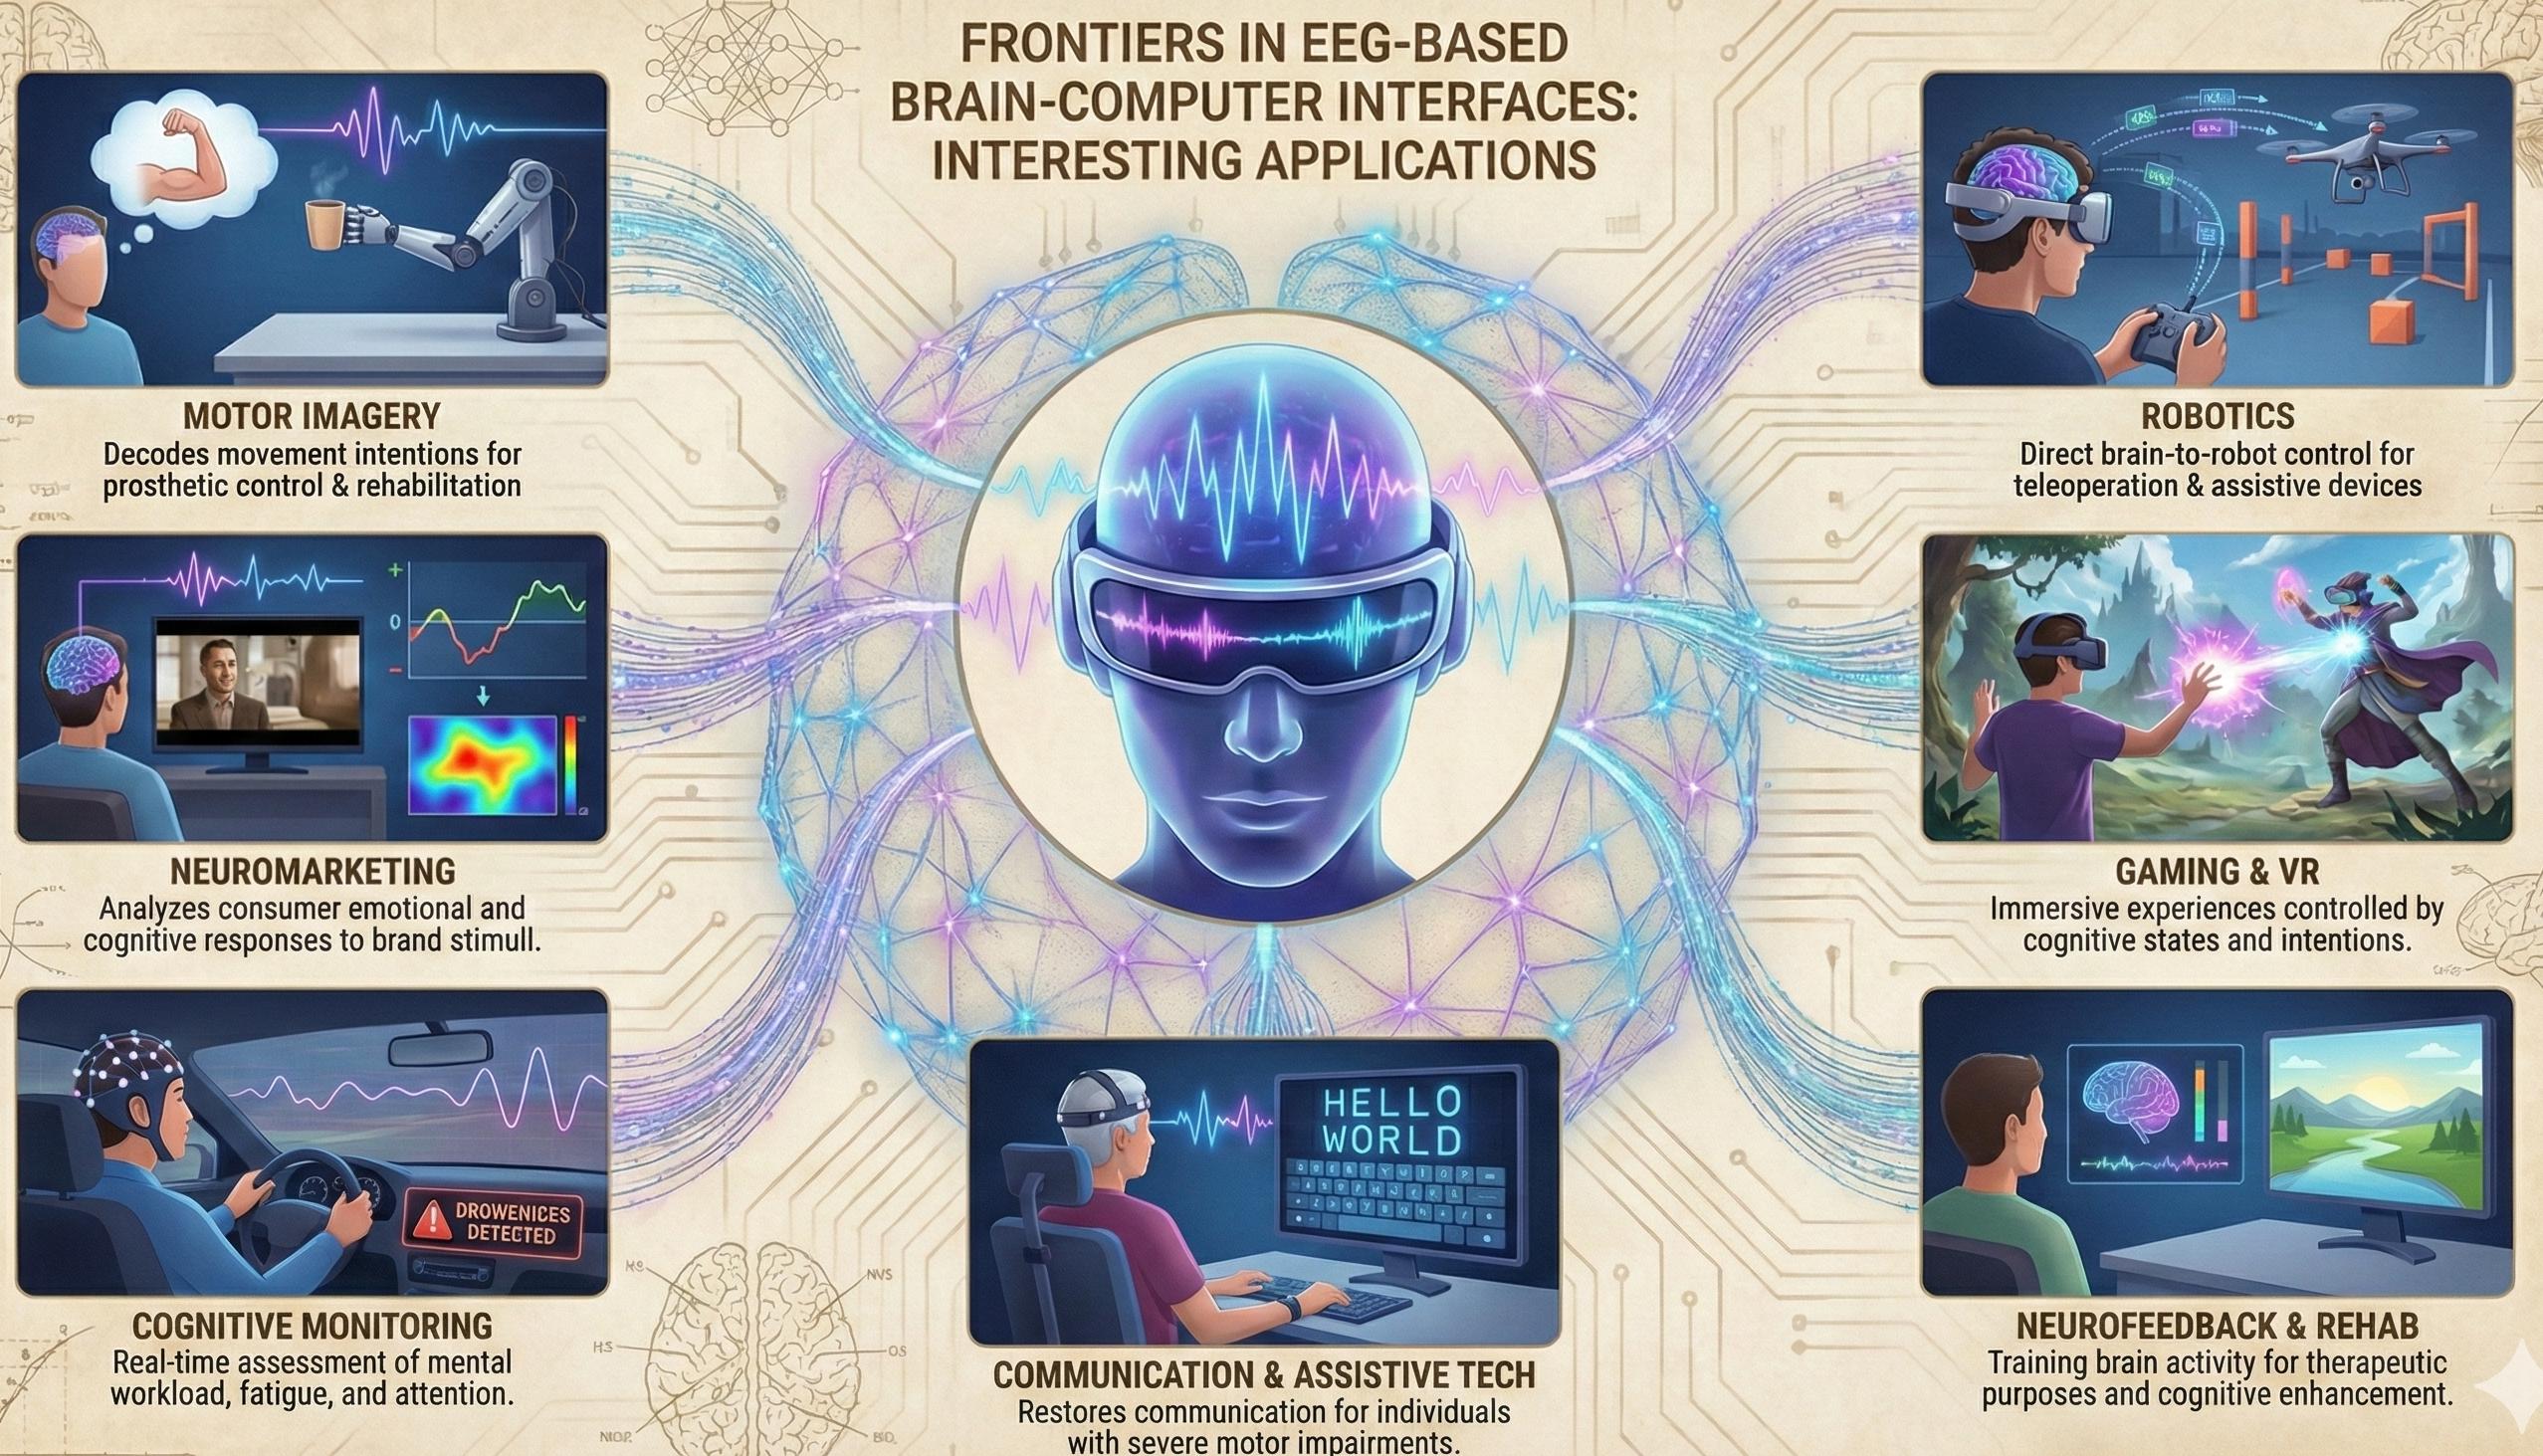
\includegraphics[width=1\textwidth]{Cap_1/Figures/Bci_apli2.png}
    \caption{Applications of EEG-based \glspl{BCI} in different domains.}
    \label{fig:BCI_aplications}
\end{figure}


Serious games are digital environments designed not solely for entertainment, but to fulfill educational, therapeutic, or cognitive objectives \cite{damavsevivcius2023serious}. In the context of neurodevelopmental disorders such as \gls{ADHD}, they have become increasingly relevant as tools for both cognitive assessment and intervention \cite{Patino2025}. Their engaging and adaptive nature allows them to target specific executive functions—like attention, inhibition, and working memory—while maintaining high user motivation, particularly among children \cite{RodriguezTimana2024}. To achieve this, two principal paradigms guide their design \cite{DeLuca2024}. The first is the task-based paradigm, which integrates classical neuropsychological tasks—such as the Go/No-Go, n-back, or Stroop test—into interactive game mechanics, allowing for the precise measurement of behavioral responses tied to well-established cognitive models \cite{Fang2025}. The second is the neurofeedback paradigm, in which the game dynamically responds to real-time EEG signals, offering auditory or visual feedback based on the user’s brain state. This paradigm supports operant conditioning mechanisms, encouraging users to self-regulate neural activity linked to attentional control and inhibition \cite{Firouzabadi2022}.

These design paradigms are intricately aligned with four core cognitive models critical to \gls{ADHD} pathology: attention, working memory, inhibition, and planning (see Figure \ref{fig:cognitive_models}). Games targeting the attentional model aim to improve sustained and selective attention, often requiring players to maintain focus amid distractions or shifting stimuli \cite{Chen2024}. Working memory is typically trained through tasks that require the temporary storage and manipulation of information, such as remembering sequences or updating mental representations. The inhibition model involves suppressing prepotent responses or resisting distractions—commonly implemented through fast-paced decision-making challenges or impulse control mechanics \cite{Takahashi2024, BreitlingZiegler2020}. Finally, the planning model emphasizes goal-directed behavior, encouraging users to sequence actions, solve multi-step problems, or anticipate future outcomes \cite{Lorini2022}. By aligning game mechanics with these cognitive models, serious games become powerful tools not only for engagement but for targeted neurocognitive intervention.

\begin{figure}[h]
    \centering
    \includegraphics[width=1\textwidth]{Cap_1/Figures/cognitive.pdf}
    \caption{Core cognitive models targeted by serious games in ADHD interventions: attention, working memory, inhibition, and planning. Each model maps to a specific set of game dynamics and EEG markers.}
    \label{fig:cognitive_models}
\end{figure}


When these targeted interventions are integrated with \gls{BCI} technology, they demonstrate substantial therapeutic benefits by reinforcing executive function, improving behavioral outcomes, and reducing symptom severity through active attention training \cite{Doulou2025}. By utilizing active \glspl{BCI}, in which users intentionally modulate their focus to influence the outcome of the game, these systems have been shown to strengthen cognitive control and promote long-term neuroplastic changes directly relevant to \gls{ADHD} pathology \cite{Cervantes2023}. Furthermore, these integrated platforms enable adaptive feedback, allowing interventions to dynamically adjust to each child's specific neurocognitive profile. Ultimately, combining robust cognitive models with real-time, objective EEG feedback makes serious games uniquely compatible with \glspl{BCI}, providing a highly personalized framework for interactive cognitive modulation.


Recent developments in portable EEG hardware have expanded the applicability of \glspl{BCI} for \gls{ADHD} beyond clinical settings, enabling real-time monitoring and feedback in homes, classrooms, and therapeutic environments (see Figure~\ref{fig:system_overview}). Low-cost, wireless EEG headsets—equipped with dry electrodes and embedded microcontrollers—have been successfully integrated into neurofeedback systems and serious games designed for children \cite{Xu2018}. These platforms allow for real-time signal acquisition and onboard processing, supporting closed-loop interventions without reliance on external computers. Thanks to ARM-based processors and system-on-chip (SoC) designs, it is now possible to run lightweight machine learning models directly on the device for real-time EEG classification \cite{Wang_2020}. Moreover, custom head-mounted EEG systems have shown reliable tracking of the theta/beta ratio, a key biomarker for \gls{ADHD}, during interactive tasks \cite{Larocco2020}.

\begin{figure}[h]
    \centering
    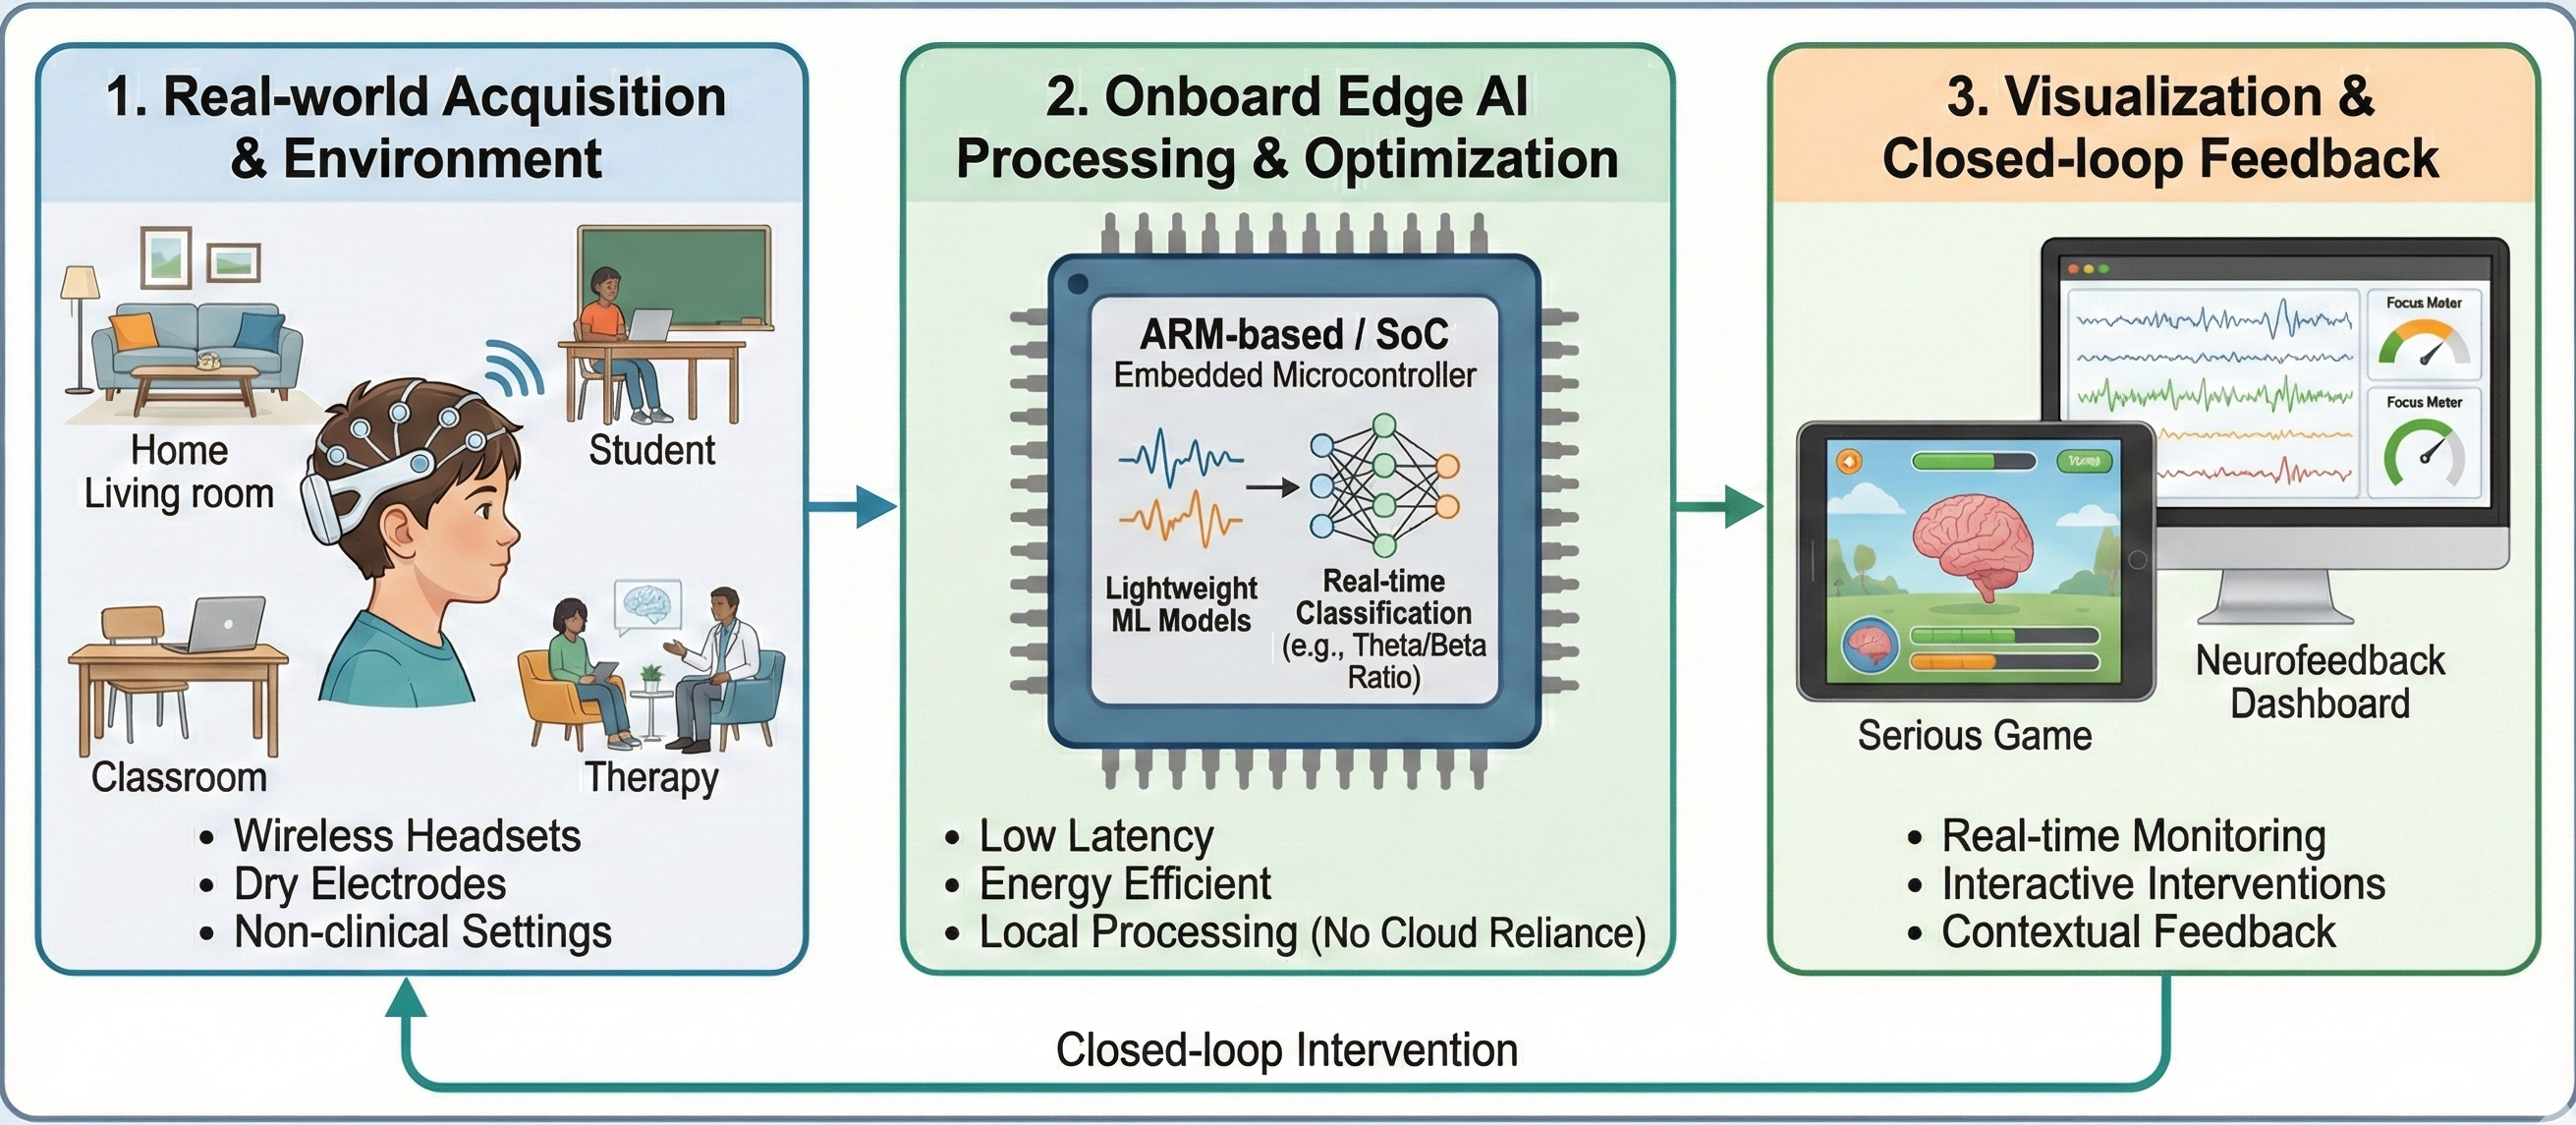
\includegraphics[width=1\textwidth]{Cap_1/Figures/BCI_IA.png}
    \caption{Overview of the Brain-Computer Interface (BCI) and Artificial Intelligence (AI) integration for neurocognitive assessment.}
    \label{fig:system_overview}
\end{figure}

The push to bring these portable, AI-driven interventions out of the clinic is heavily supported by the rapid expansion of the digital health sector. As of 2024, the global telehealth and telemedicine market surpassed \$123 billion, reflecting a permanent shift toward decentralized care and remote patient monitoring \cite{grandview_telehealth_2024}. To support this transition, the global embedded systems market reached over \$112 billion in 2024, driven by an immense demand for compact, energy-efficient Internet of Medical Things (IoMT) devices \cite{coherent_embedded_2024}. Concurrently, the integration of artificial intelligence into healthcare—a market valued at over \$13 billion in the U.S. alone in 2024—demonstrates a strong clinical and commercial drive to embed complex diagnostic intelligence directly into everyday environments \cite{novaone_ai_healthcare_2024}. These economic indicators highlight a clear motivation: there is a profound necessity to translate hospital-grade capabilities into accessible, wearable form factors that operate autonomously.

To successfully deploy these autonomous systems in daily life, research must focus on optimizing hardware and software integration for strict portable constraints \cite{phiri2023adaptive}. Operating continuously in non-clinical settings necessitates highly efficient energy and resource use, as wearable devices are bound by severe power and memory limitations. Processing biosignals locally via edge AI reduces latency and power-heavy cloud transmissions, yet it requires highly tailored acquisition algorithms that maximize computational efficiency \cite{shajari2023emergence}. Furthermore, capturing a comprehensive physiological profile demands the precise synchronization of biomarkers across distributed sensors \cite{ramasubramanya2025wearable}. Ensuring that multi-modal data streams are temporally aligned is an absolute necessity for generating accurate, real-time contextual feedback. By establishing robust methods to efficiently acquire, align, and process these integrated biomarkers on low-power architectures, this research aims to unlock the full therapeutic potential of continuous, closed-loop neurofeedback outside of traditional medical facilities \cite{li2023application}.



To address these evolving requirements for decentralized mental health technology, this research is developed within the framework of the project called ``Alianza científica con enfoque comunitario para mitigar brechas de atención y manejo de trastornos mentales relacionados con impulsividad en Colombia'' (\gls{ACEMATE}) (Multimodal system supported by serious games for personalized neurocognitive assessment and intervention in impulsivity disorders associated with ADHD), a collaborative initiative involving the Universidad Nacional de Colombia and the Universidad Tecnológica de Pereira. \gls{ACEMATE} aims to facilitate both face-to-face and remote interventions across clinical, educational, and community settings. However, realizing this vision of accessible care relies entirely on deploying physical infrastructure that resolves the previously outlined technical bottlenecks—specifically, the need for robust, portable hardware capable of precise biomarker synchronization. Consequently, this thesis proposes the development of MONEEE, a specialized EEG signal acquisition system designed to serve as the hardware enabler for \gls{ACEMATE}. By ensuring low-latency marker integration and high signal fidelity under strict energy and resource constraints, MONEEE provides the essential technological foundation to power the broader \gls{ACEMATE} ecosystem, ultimately democratizing access to objective, technology-driven mental health services for children.

\begin{figure}[h]
    \centering
    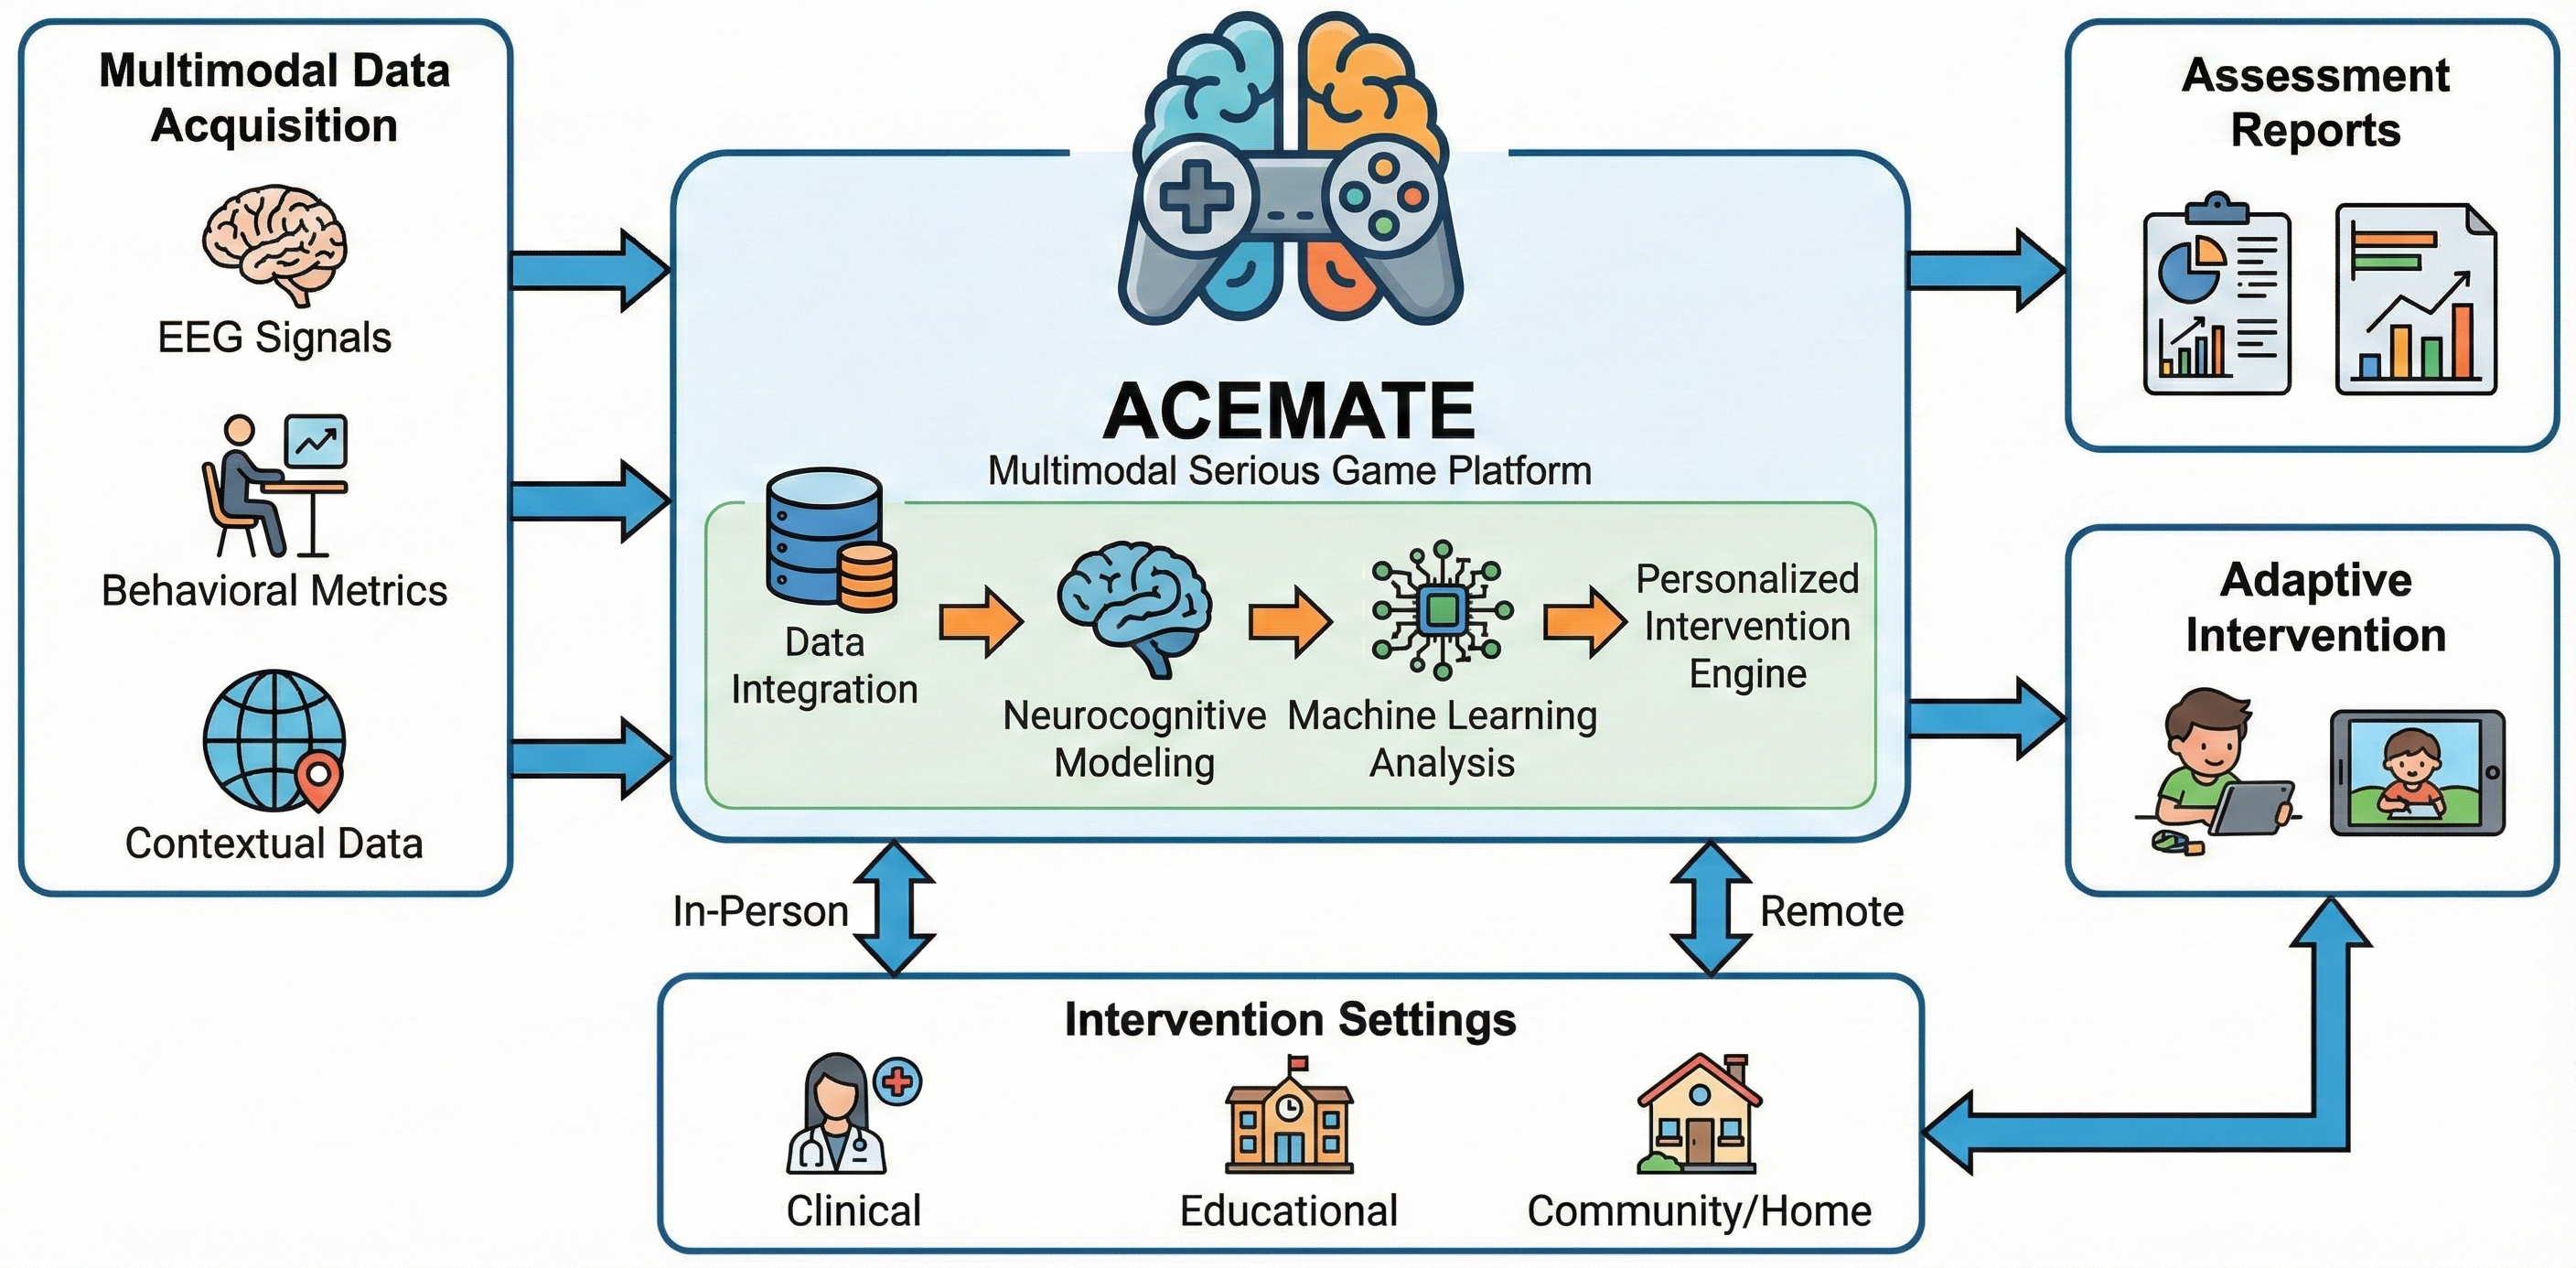
\includegraphics[width=1\textwidth]{Cap_1/Figures/acemate.png}
    \caption{Overview of the \gls{ACEMATE} project.}
    \label{fig:acemate}
\end{figure}



\section{Problem statement}
\label{sec:problem}

While the integration of BCIs and continuous \gls{EEG} monitoring within serious games presents a promising avenue for neurocognitive assessment, translating these concepts into functional clinical tools requires a highly robust underlying hardware architecture \cite{craik2023design}. Fundamentally, the physical acquisition of this neural data begins with an \gls{EEG} cap fitted with non-invasive sensors designed to detect microvolt-level electrical signals from the cerebral cortex. Because these raw biological signals are inherently weak and highly susceptible to noise, they must be routed to a dedicated acquisition board or a multi-stage card system \cite{armand2024low}. This hardware typically consists of an analog front-end—responsible for the high-precision amplification, filtering, and digitization of the signals—and a digital processing unit, such as a microcontroller, for real-time data management and routing \cite{janapati2023advances}. To effectively map the neurocognitive responses elicited by the serious games, this continuous neural data must be contextually locked to specific in-game cognitive stimuli. This vital synchronization is achieved by interfacing the acquisition hardware with the stimulus presentation device, which transmits discrete event markers that map external gameplay milestones directly to the \gls{EEG} stream \cite{minissi2025role}.

However, the translation of this theoretical promise into clinical reality faces formidable engineering barriers. The efficacy of closed-loop interventions is predicated not on the mere availability of data, but on the fidelity and temporal determinism of that data \cite{sabio2024scoping}. Current acquisition architectures, particularly those designed for portability and low cost, are frequently plagued by systemic failures that sever the causal link between neural intention and digital response \cite{ariza2022low}. This research defines and analyzes two such sequential, critical failures. The foundational challenge stems from severe Signal-to-Noise Ratio (\gls{SNR}) limitations inherent to embedded architectures \cite{li2025high}. In portable \gls{EEG} devices designed for \gls{ADHD} monitoring, the physical proximity of high-speed digital processing components inevitably introduces electromagnetic interference. This interference degrades the system's high-precision analog sensing, corrupting the delicate microvolt-level neural signals required before any valid clinical evaluation can even begin \cite{dobrev2022high}. Once a reliable physiological signal is secured, a second, equally critical failure emerges: the precise synchronization of biomarkers \cite{esteban2026synchronization}. Because \gls{ADHD} neurocognitive assessments rely heavily on time-locked neural responses to specific game events, any temporal variability or unpredictable latency between the digital stimuli and the recorded biological signals fundamentally compromises the diagnostic validity of the data \cite{kaminski2026complexity}. The contrast between the theoretical promise of continuous monitoring and the clinical reality is summarized in Figure \ref{fig:general_barriers}.


\begin{figure}[h]
    \centering
    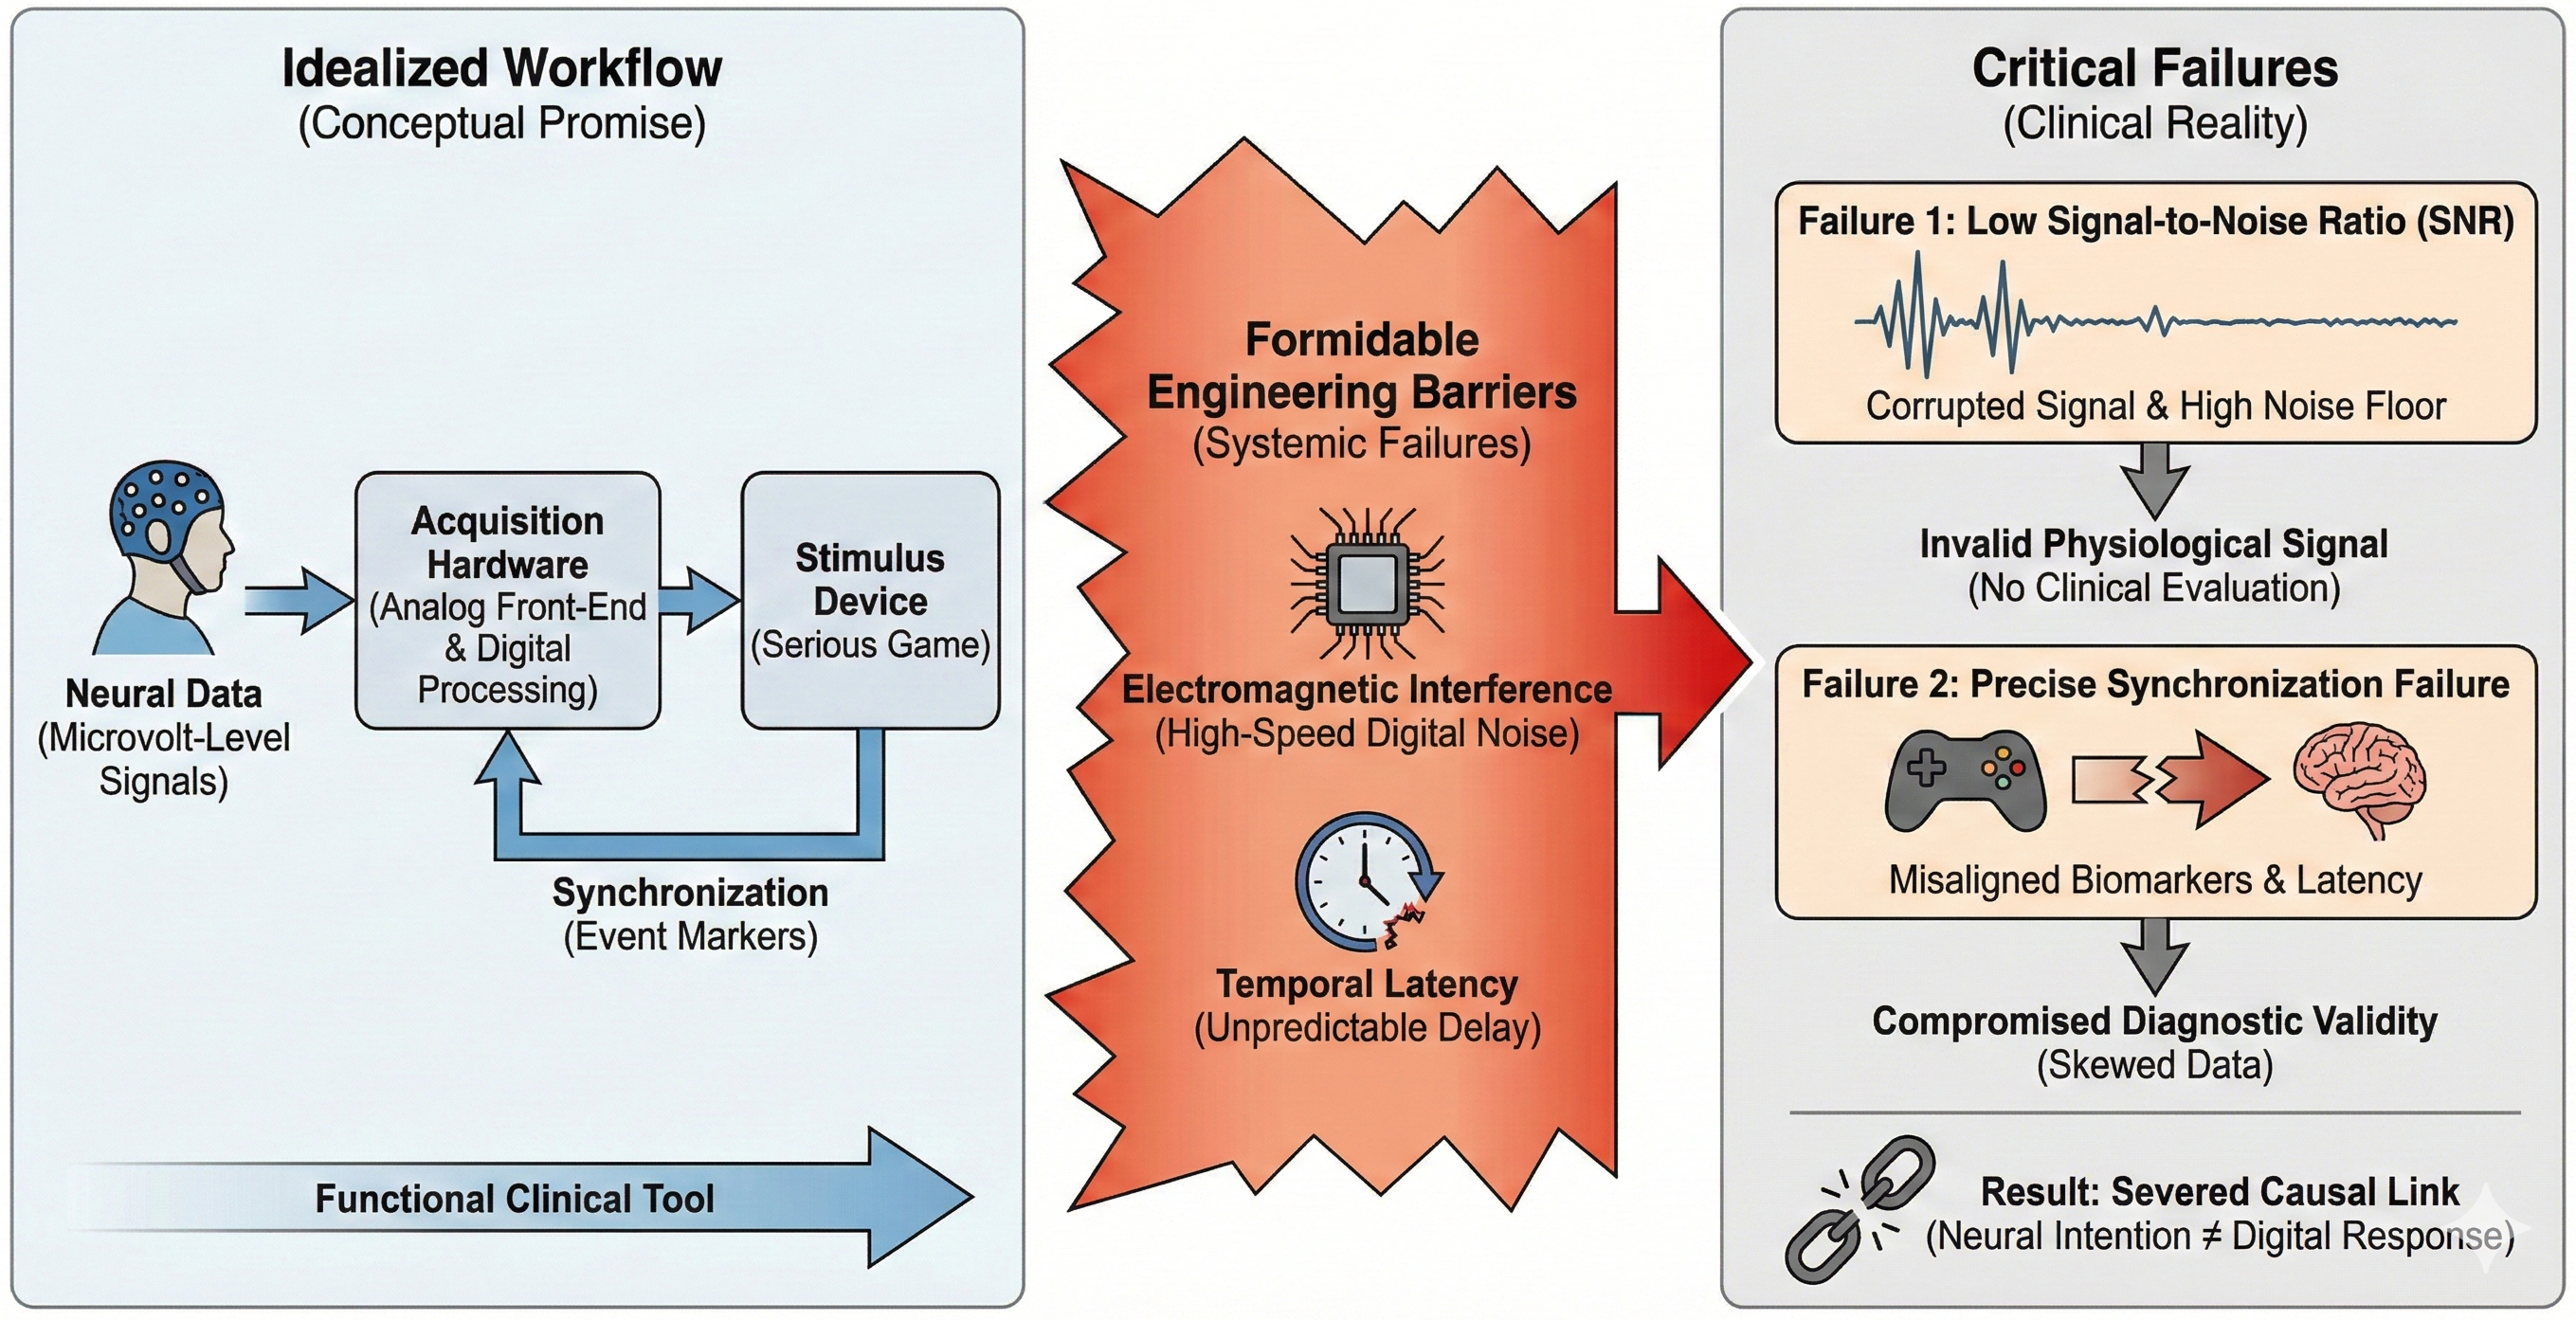
\includegraphics[width=0.8\linewidth]{Cap_1/Figures/Problem_general.png}
    \caption{The clinical translation problem in neurocognitive assessment systems. The illustration defines the two sequential critical failures that compromise diagnostic validity: the corruption of the analog signal and the temporal misalignment of biomarkers.}
    \label{fig:general_barriers}
\end{figure}


\subsection{SNR limitations in embedded systems}


The physical interface of traditional clinical EEG setups creates a major operational bottleneck for pediatric neurocognitive assessment. Lengthy and restrictive cap placement processes consistently induce restlessness, anxiety, and movement artifacts in children with ADHD \cite{Lim2023}. If the acquisition hardware cannot be deployed rapidly and comfortably, the resulting setup latencies and prolonged impedance stabilization times severely degrade the \gls{SNR} \cite{gorjan2022removal}. This physical friction directly compromises the ecological validity and engagement required for a serious game environment, making the rapid deployment of the acquisition cap a critical challenge to overcome \cite{kaongoen2023future}.

Once the physical interface is established, preserving analog signal integrity within a densely populated, mixed-signal embedded system presents a fundamental hardware challenge \cite{liu2024design}. The close physical proximity of high-speed digital processing units to the analog front-end introduces severe risks of electromagnetic interference and power supply noise coupling \cite{devi2022survey}. If physical board layout and isolation strategies are inadequate, the system's intrinsic background noise will inevitably exceed the baseline input-referred noise thresholds of the acquisition components (typically 1 µVpp) \cite{rashid2018eeg}. Overcoming this mixed-signal noise ceiling is essential; failure to do so creates a high noise floor that completely masks the low-amplitude Event-Related Potentials (\glspl{ERP}) necessary for cognitive assessment \cite{kim2022miniaturization}.

Even if analog noise is successfully mitigated, the embedded system's processing hardware faces severe resource constraints when managing continuous, high-frequency electrophysiological data streams. Unoptimized continuous data logging demands substantial computational power and can rapidly induce I/O bottlenecks, RAM saturation, and subsequent thermal throttling \cite{battaglia2022eeg}. The immediate consequence of an overburdened CPU or saturated memory footprint is the dropping of crucial data packets and the introduction of variable acquisition latency \cite{arroba2024sustainable}. This resource exhaustion fundamentally corrupts the integrity and continuity of the EEG data stream itself. Therefore, continuous monitoring of RAM usage and CPU load is critical to ensure the hardware can sustain reliable, uninterrupted data acquisition without buckling under the operational demands \cite{ajmeria2022critical}. As illustrated in Figure \ref{fig:hardware_bottlenecks}, the physical friction of traditional cap placement and the subsequent risk of analog signal corruption present immediate hurdles.


\begin{figure}[h]
    \centering
    \includegraphics[width=0.8\linewidth]{Cap_1/Figures/subproblem1.png}
    \caption{Physical, electrical, and computational resource barriers in deploying \gls{EEG} systems. The illustration highlights operational bottlenecks during patient setup, the risk of \gls{SNR} degradation due to mixed-signal interference, and embedded system resource exhaustion.}
    \label{fig:hardware_bottlenecks}
\end{figure}

\subsection{Synchronization and temporal variability in \gls{EEG} biomarkers}

The primary challenge in extracting valid neurocognitive assessments lies in the precise temporal synchronization of acquired \gls{EEG} biomarkers with external serious game stimuli \cite{ahmed2025eeg}. During interactive sessions, event markers are continuously transmitted from the game interface to the acquisition system. Standard communication protocols, however, introduce inherent, non-deterministic latency driven by transmission overhead, variable polling rates, and operating system scheduling conflicts \cite{buraimoh2023overview}. This unpredictable communication jitter fundamentally skews the temporal alignment between the stimulus presented to the patient and the corresponding neurophysiological response \cite{larsen2024method}. By conducting rigorous short-term latency bounding tests, this immediate communication delay must be quantified and mitigated to ensure the calculated Event-Related Potentials (ERPs) are temporally accurate and clinically viable \cite{he2023diversity}.

Beyond the immediate delay of single events, maintaining precise synchronization throughout a complete clinical session presents a compounding temporal challenge. Standard pediatric ADHD evaluations demand sustained, uninterrupted engagement. Continuous execution over these extended periods exposes the acquisition architecture to cumulative temporal errors \cite{arpaia2025acquisition}. Asynchronous clock drift between the event triggers and the hardware sampling rate, coupled with potential memory buffer saturation and thermal-induced performance fluctuations, introduces progressive instability \cite{dasenbrock2022synchronization}. This compounding jitter degrades deterministic data throughput, leading to a critical flaw where an ERP captured at the end of a session exhibits a fundamentally different latency profile than one captured at the beginning. Extended stability testing over full-length sessions is therefore imperative to prevent temporal degradation and validate the long-term reliability of the continuous EEG stream \cite{tran2026inter}.

In parallel with resolving these mechanical timing issues, valid synchronization relies on the system's proven ability to capture authentic, dynamic electrophysiological phenomena rather than structured noise \cite{correia2024brain}. Before complex ERPs can be reliably synchronized with external events, a foundational physiological baseline test must be conducted. This problem is addressed by detecting spontaneous frequency modulations, specifically the well-documented attenuation of alpha-band activity (8–13 Hz) when a subject transitions from an eyes-closed to an eyes-open state \cite{isler2023longitudinal}. If the signal processing pipeline distorts the bandwidth or lacks the sensitivity to capture these baseline spectral shifts, the recorded data is physiologically invalid \cite{flo2022automated}. Verifying the fundamental ability to resolve these basic frequency changes ensures that the synchronized event markers are anchored to genuine neural activity \cite{frelih2025modulation}. Figure \ref{fig:sync_challenges} demonstrates how non-deterministic latency and cumulative temporal drift fundamentally skew the alignment between the game stimulus and the neurophysiological response.

Finally, the temporal precision of the biomarkers must be matched by their spatial and structural integrity, which requires addressing inherent hardware vulnerabilities. High-resolution, multi-channel EEG acquisition creates a strict physical requirement for trace isolation to prevent analog signal bleed. Without meticulous shielding, adjacent channels inevitably suffer from crosstalk, blending distinct spatial brain waves and destroying the topographical accuracy of the recorded data. Furthermore, rendering these continuous data streams can introduce visualization artifacts that masquerade as genuine visual transients or \glspl{ERP}. By executing rigorous signal isolation and artifact detection tests, these structural issues can be identified and eliminated, ensuring that the precisely synchronized neurocognitive markers are extracted from pristine, uncontaminated data.



\begin{figure}[h]
    \centering
    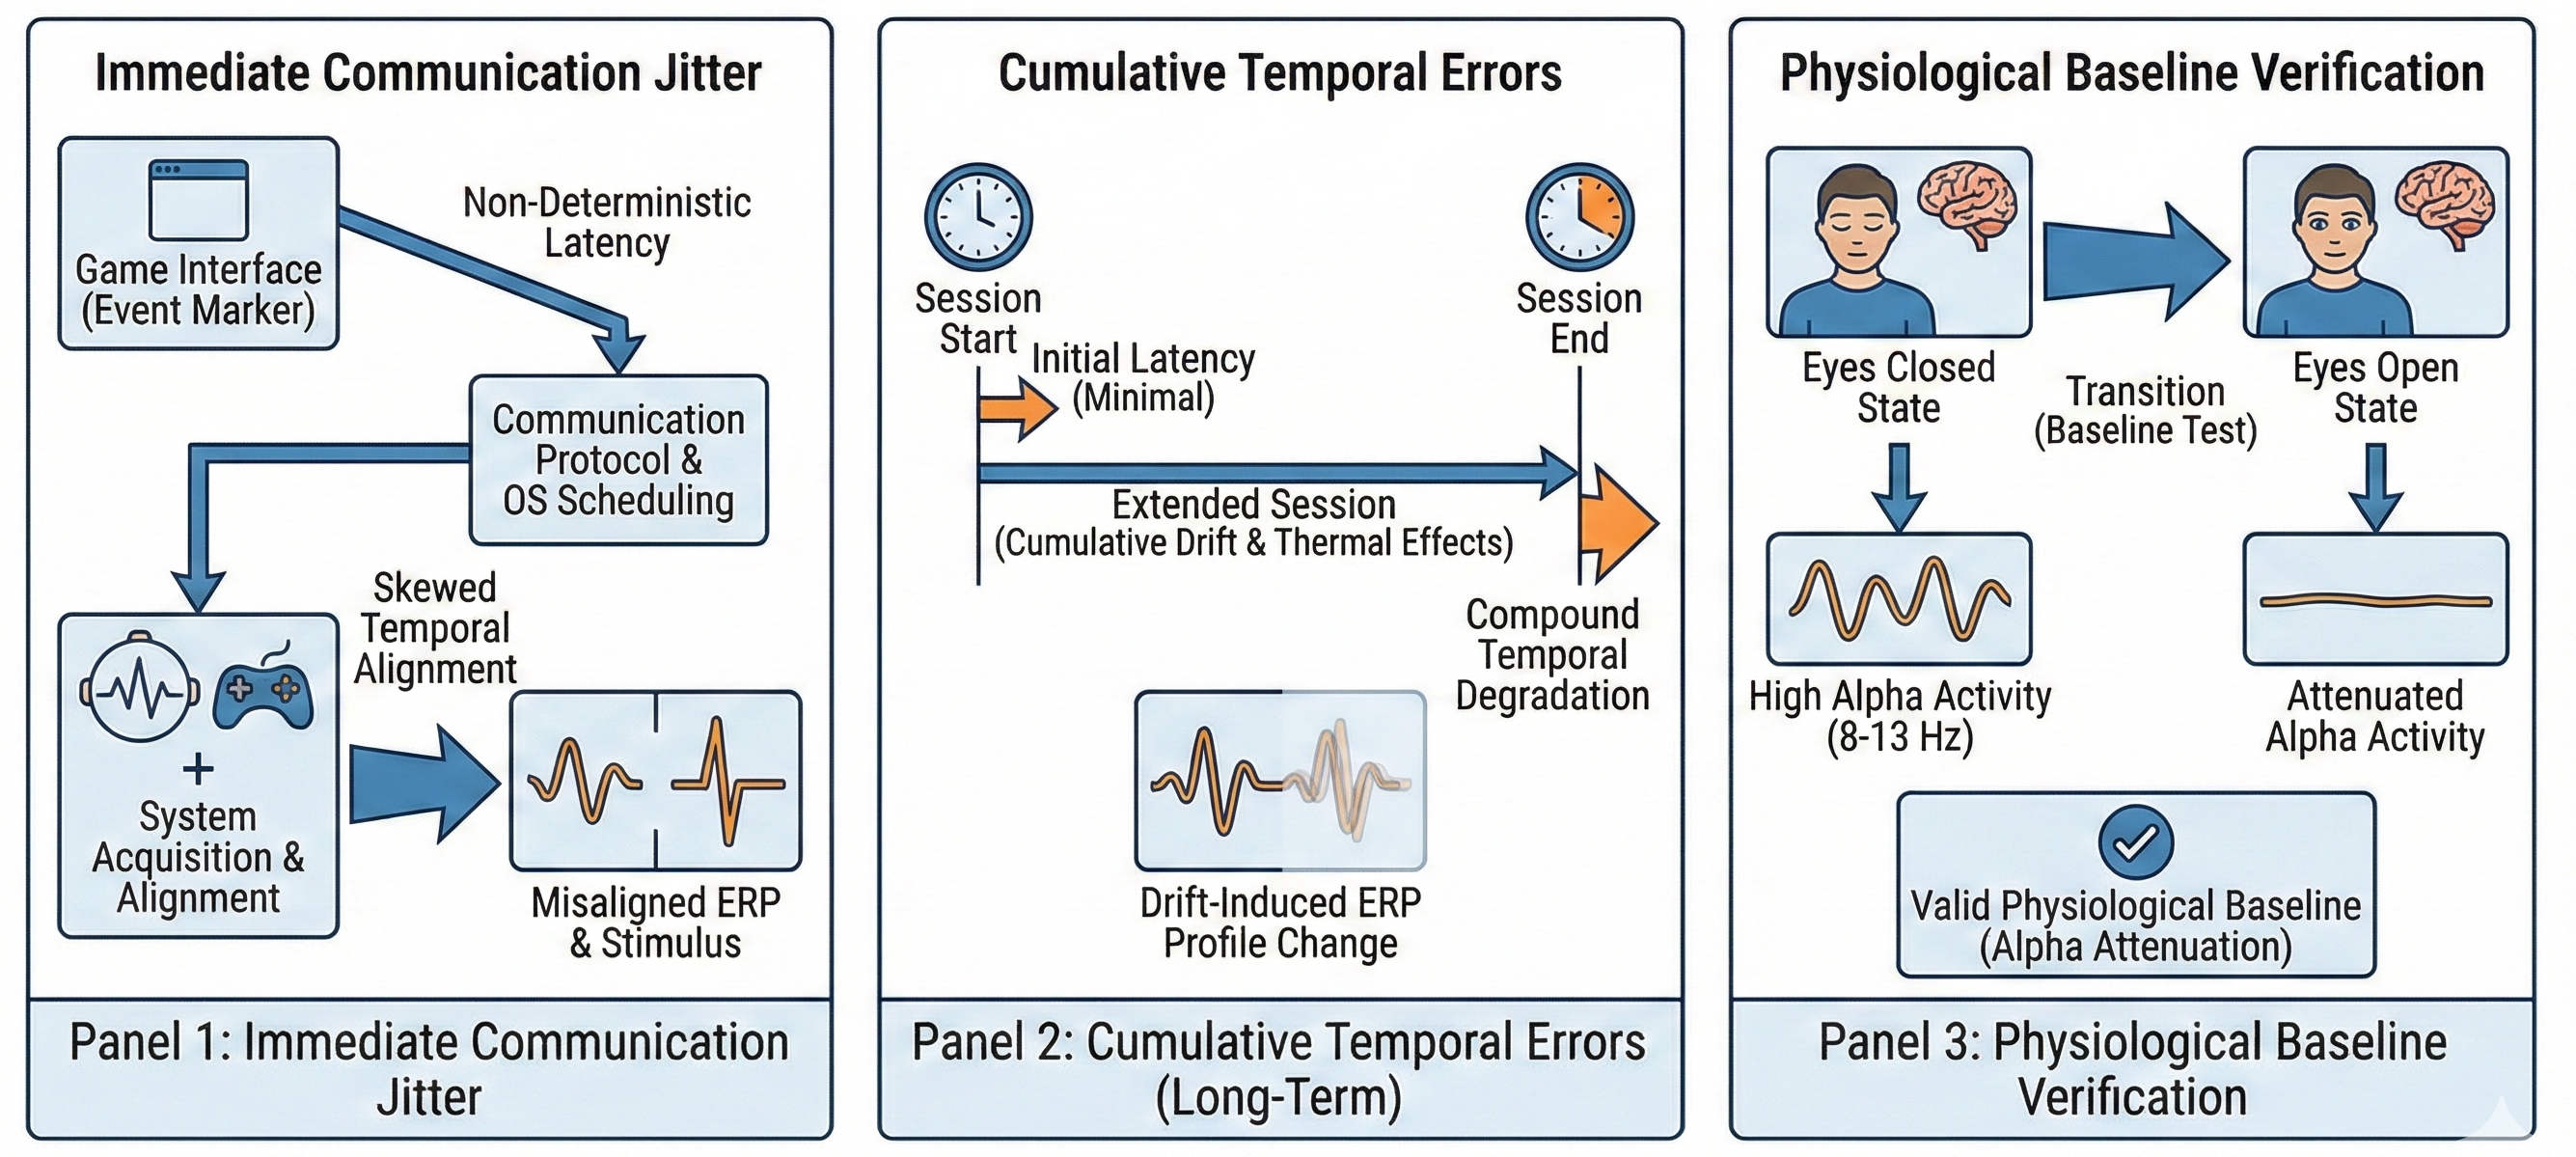
\includegraphics[width=0.8\linewidth]{Cap_1/Figures/subproblem2.png}
    \caption{Synchronization errors and real-time physiological validation. This figure details the impact of short-term non-deterministic communication jitter, cumulative temporal drift in extended sessions, and physiological baseline verification via alpha-band attenuation.}
    \label{fig:sync_challenges}
\end{figure}





\newpage
\section{Research question}\label{sec:question}

How can an embedded EEG acquisition architecture be optimized to simultaneously mitigate mixed-signal interference and non-deterministic synchronization jitter to ensure the clinical validity of biomarkers in serious-game-based ADHD assessments?



\section{State of art}\label{sec:stateofart}


In recent years, numerous wireless systems for EEG data acquisition have been developed, with two main approaches standing out: conventional remote monitoring systems and portable smart systems. The former simply digitize the EEG signals and transmit them to a remote unit for processing, usually in a deferred manner \cite{arpaia2020wearable}. On the other hand, portable systems preprocess the signals on a local device, such as a microcontroller (MCU), and wirelessly transmit the data using low-power consumption protocols. \ref{table:bci_hardware} This latter approach is crucial for real-time applications, where low latency is essential.

Marker synchronization in portable EEG acquisition systems \cite{razavi2022opensync}, particularly in applications combined with serious games \cite{damavsevivcius2023serious}, faces several technical and operational challenges. One of the main issues lies in latency in data transmission protocols. In portable EEG systems, precise synchronization between brain events and interactions in the game is crucial \cite{gomezromero2024implications}, but inherent limitations of portable acquisition systems, such as latencies in data transfer protocols, can cause temporal mismatches. These latencies primarily stem from bandwidth constraints in wireless transmission and the need to process large volumes of data in real-time \cite{he2023diversity}.

The type of electrode \cite{liu2023feature} and the number of channels \cite{abdullah2022eeg}  are determining factors in the quality of the data acquired in portable systems. Although dry electrodes offer greater portability, they tend to generate lower-quality signals due to reduced conductivity, which can complicate precise synchronization with other devices, such as serious games. On the other hand, the use of systems with \textbf{low channel density (e.g., 8-16 channels)} \cite{allouch2023effect} is a common strategy in these portable systems to minimize size and improve portability. However, low channel density can affect the spatial resolution of EEG data, limiting the ability to perform accurate analysis of brain patterns. This challenge is reflected in the need to optimize sampling \cite{zheng2023effects}  and data transfer protocols \cite{bayilmics2022survey}  to ensure that captured signals are transmitted efficiently without significant information loss

The sampling rate is another critical factor, as it directly affects the temporal resolution of EEG signals. The combination of low channel density and insufficient sampling rate can make it difficult to capture fast brain events, such as attention shifts, which are essential in applications like serious games. Furthermore, Signal Front-End Amplifiers (AFE) \cite{devi2022survey} play a key role in signal quality. While low-cost AFEs may be suitable for portable systems, they tend to have limitations in processing capacity, which impacts data synchronization by generating noise and distortions in the EEG signals, especially when connected to mobile devices with lower processing power.

Battery life \cite{niso2023wireless} is a significant constraint for portable systems that require long monitoring sessions. EEG systems that operate for several hours often need to optimize their energy consumption, which may involve reducing the sampling rate or channel density, once again impacting data quality and real-time synchronization.


\begin{table}[H]
    \caption{Acquisition devices used for BCI. The table provides an overview of the different hardware devices, their specifications, and communication protocols.}
    \label{table:bci_hardware}
    \centering
    \footnotesize
    \begin{tabularx}{\textwidth}{|X|p{1.8cm}|p{1.8cm}|c|>{\centering\arraybackslash}X|c|X|c|}
        \hline
        \textbf{Hardware BCI} & \textbf{Empresa} & \textbf{Tipo de Electrodo} & \textbf{Canales} & \textbf{Frecuencia de Muestreo} & \textbf{AFE} & \textbf{Protocolo y Transferencia} & \textbf{Batería} \\ \hline
        Cyton + Daisy \cite{OpenBCI_CytonDaisy} & OpenBCI & Flexible / Húmedo / Seco & 16 & 250 Hz - 16 kHz & ADS1299 & RF / BLE / Wi-Fi & 8 h \\ \hline
        actiCAP \cite{BrainProducts_ActiCap} & Brain Products GmbH & Flexible / Húmedo / Seco & 16 & 256 Hz - 16 kHz & - & USB & 16 h \\ \hline
        EPOC X \cite{Emotiv_EPOCX} & Emotiv & Rígido / Húmedo & 14 & 128 Hz & - & BLE / Bluetooth & 6--12 h \\ \hline
        Diadem \cite{Bitbrain_Diadem} & Bitbrain & Rígido / Seco & 12 & 256 Hz & - & Bluetooth & 8 h \\ \hline
        g.Nautilus \cite{Gtec_GNautilusProFlexible} & g.tec & Flexible & 8 / 16 / 32 & 250 Hz & ADS1299 & Propietario & 10 h \\ \hline
        Plataforma para EEG ambulatorio \cite{pinho2014wireless} & - & Activo / Seco & 32 & 250 Hz- -1 kHz & ADS1299 & Wi-Fi 802.11 b/g/n & 26 h \\ \hline
        Sistema para neurofeedback \cite{Totev2023} & - & Pasivo / Seco & 40 & 250 Hz & ADS1298 & RF & - \\ \hline
        BEATS \cite{Beats} & - & Flexible / Húmedo & 32 & 4 kHz & ADS1299 & Wi-Fi & 24 h (cableado) \\ \hline
    \end{tabularx}
\end{table}




In the field of brain-computer interfaces (BCIs), several devices have been developed, each with unique features tailored to specific use cases such as clinical research, neurofeedback, or consumer applications. The Cyton + Daisy system by OpenBCI \cite{OpenBCI_CytonDaisy} supports up to 16 channels and offers a wide sampling rate range of 250 Hz to 16 kHz, making it suitable for high-resolution EEG acquisition. The device uses flexible, wet, or dry electrodes and incorporates the ADS1299 AFE for high-quality signal conversion. It supports data transfer via RF, Bluetooth Low Energy (BLE), and Wi-Fi, allowing for versatile connectivity. With a battery life of 8 hours, this system is highly adaptable, suitable for both research and practical applications in various environments. Another system, actiCAP \cite{BrainProducts_ActiCap} by Brain Products GmbH, features flexible, wet, or dry electrodes and is capable of recording up to 16 channels with a sampling rate range from 256 Hz to 16 kHz. The actiCAP does not use a dedicated AFE and instead relies on a USB protocol for data transfer. The device provides a robust 16-hour battery life, making it an ideal choice for long-duration experiments and clinical settings that require stable signal acquisition over extended periods. The EPOC X \cite{Emotiv_EPOCX} by Emotiv is a more compact and consumer-oriented BCI device that uses rigid, wet electrodes and supports 14 channels with a sampling rate of 128 Hz. This device employs Bluetooth Low Energy (BLE) for wireless data transfer, and its battery life ranges from 6 to 12 hours, depending on usage. While its lower sampling rate may limit its use for high-resolution research, the EPOC X remains a popular choice for applications in neurofeedback, cognitive training, and general user interaction. The Diadem \cite{Bitbrain_Diadem} system by Bitbrain uses rigid, dry electrodes and supports 12 channels with a sampling rate of 256 Hz. It operates via Bluetooth for data transmission and has a battery life of 8 hours, providing a balance between portability and signal quality. The g.Nautilus \cite{Gtec_GNautilusProFlexible} system by g.tec offers great flexibility, supporting configurations with 8, 16, or 32 channels. It operates at a sampling rate of 250 Hz and uses the ADS1299 AFE for high-performance signal acquisition. The system is known for its proprietary data transmission protocol, ensuring reliable connectivity, and its battery lasts up to 10 hours, making it suitable for long-term monitoring and research studies. The BCI system used by \cite{pinho2014wireless} employs active, dry electrodes and supports up to 32 channels with a sampling rate range of 250 Hz to 1 kHz. It also incorporates the ADS1299 AFE for analog-to-digital conversion, ensuring high fidelity in signal capture. Data is transferred via Wi-Fi 802.11 b/g/n, enabling flexible and high-speed communication with external devices. The system boasts an impressive 26-hour battery life, making it an excellent option for extended usage in field studies or clinical applications. The BCI system described by \cite{Totev2023} uses passive, dry electrodes and supports up to 40 channels with a sampling rate of 250 Hz. It incorporates the ADS1298 AFE for high-quality data acquisition and utilizes RF (Radio Frequency) for data transfer. While battery life details are not specified, this device is likely designed for portable, research-focused applications where wireless data transfer is essential for real-time monitoring. Finally, the \cite{Beats} system features 32 flexible, wet electrodes and uses the ADS1299 AFE for high-precision EEG signal acquisition at a sampling rate of 4 kHz. Data is transmitted wirelessly via Wi-Fi, allowing for real-time data monitoring and analysis. The system’s battery life is 24 hours when wired, providing extended operation for intensive studies or clinical assessments that require continuous monitoring.

Each of these devices represents a different approach to EEG signal acquisition, offering varying numbers of channels, electrode types, sampling rates, and battery life. While some are optimized for research and clinical use with high sampling rates and extended battery life, others are more suited to consumer applications with lower sampling rates and shorter operational times. The choice of device depends largely on the specific needs of the user, whether for research, clinical monitoring, or personal use in neurofeedback and cognitive training applications.




%\subsection{Evolution of Portable High-Fidelity EEG Architectures}

%\subsection{Synchronization Paradigms: The "Jitter" Problem in Neurogaming}
\section{Objectives}

\subsection{General Objective}
To design and implement an EEG signal acquisition architecture optimized for applications in educational and clinical settings, focused on latency reduction and precise event synchronization, to improve the objective assessment of cognitive and emotional patterns in children with ADHD.

\subsection{Specific Objectives}
\begin{enumerate}
    \item Analyze the technical limitations of current EEG acquisition systems, including transmission latencies and low channel density.
    \item Develop low-latency algorithms and temporal synchronization strategies to ensure precise alignment between serious game stimuli and EEG responses.
    \item Evaluate the proposed architecture in clinical and educational settings, verifying its effectiveness in the diagnosis and treatment of ADHD.
\end{enumerate}

\section{Contributions and Thesis Outline}
\label{sec:contributions_outline}

In the following, we briefly introduce the main contributions of this thesis addressing the clinical translation challenges of continuous neurocognitive assessments in pediatric \gls{ADHD}. They are summarized in Figure \ref{fig:contributions}.

\begin{figure}[htpb]
    \centering
    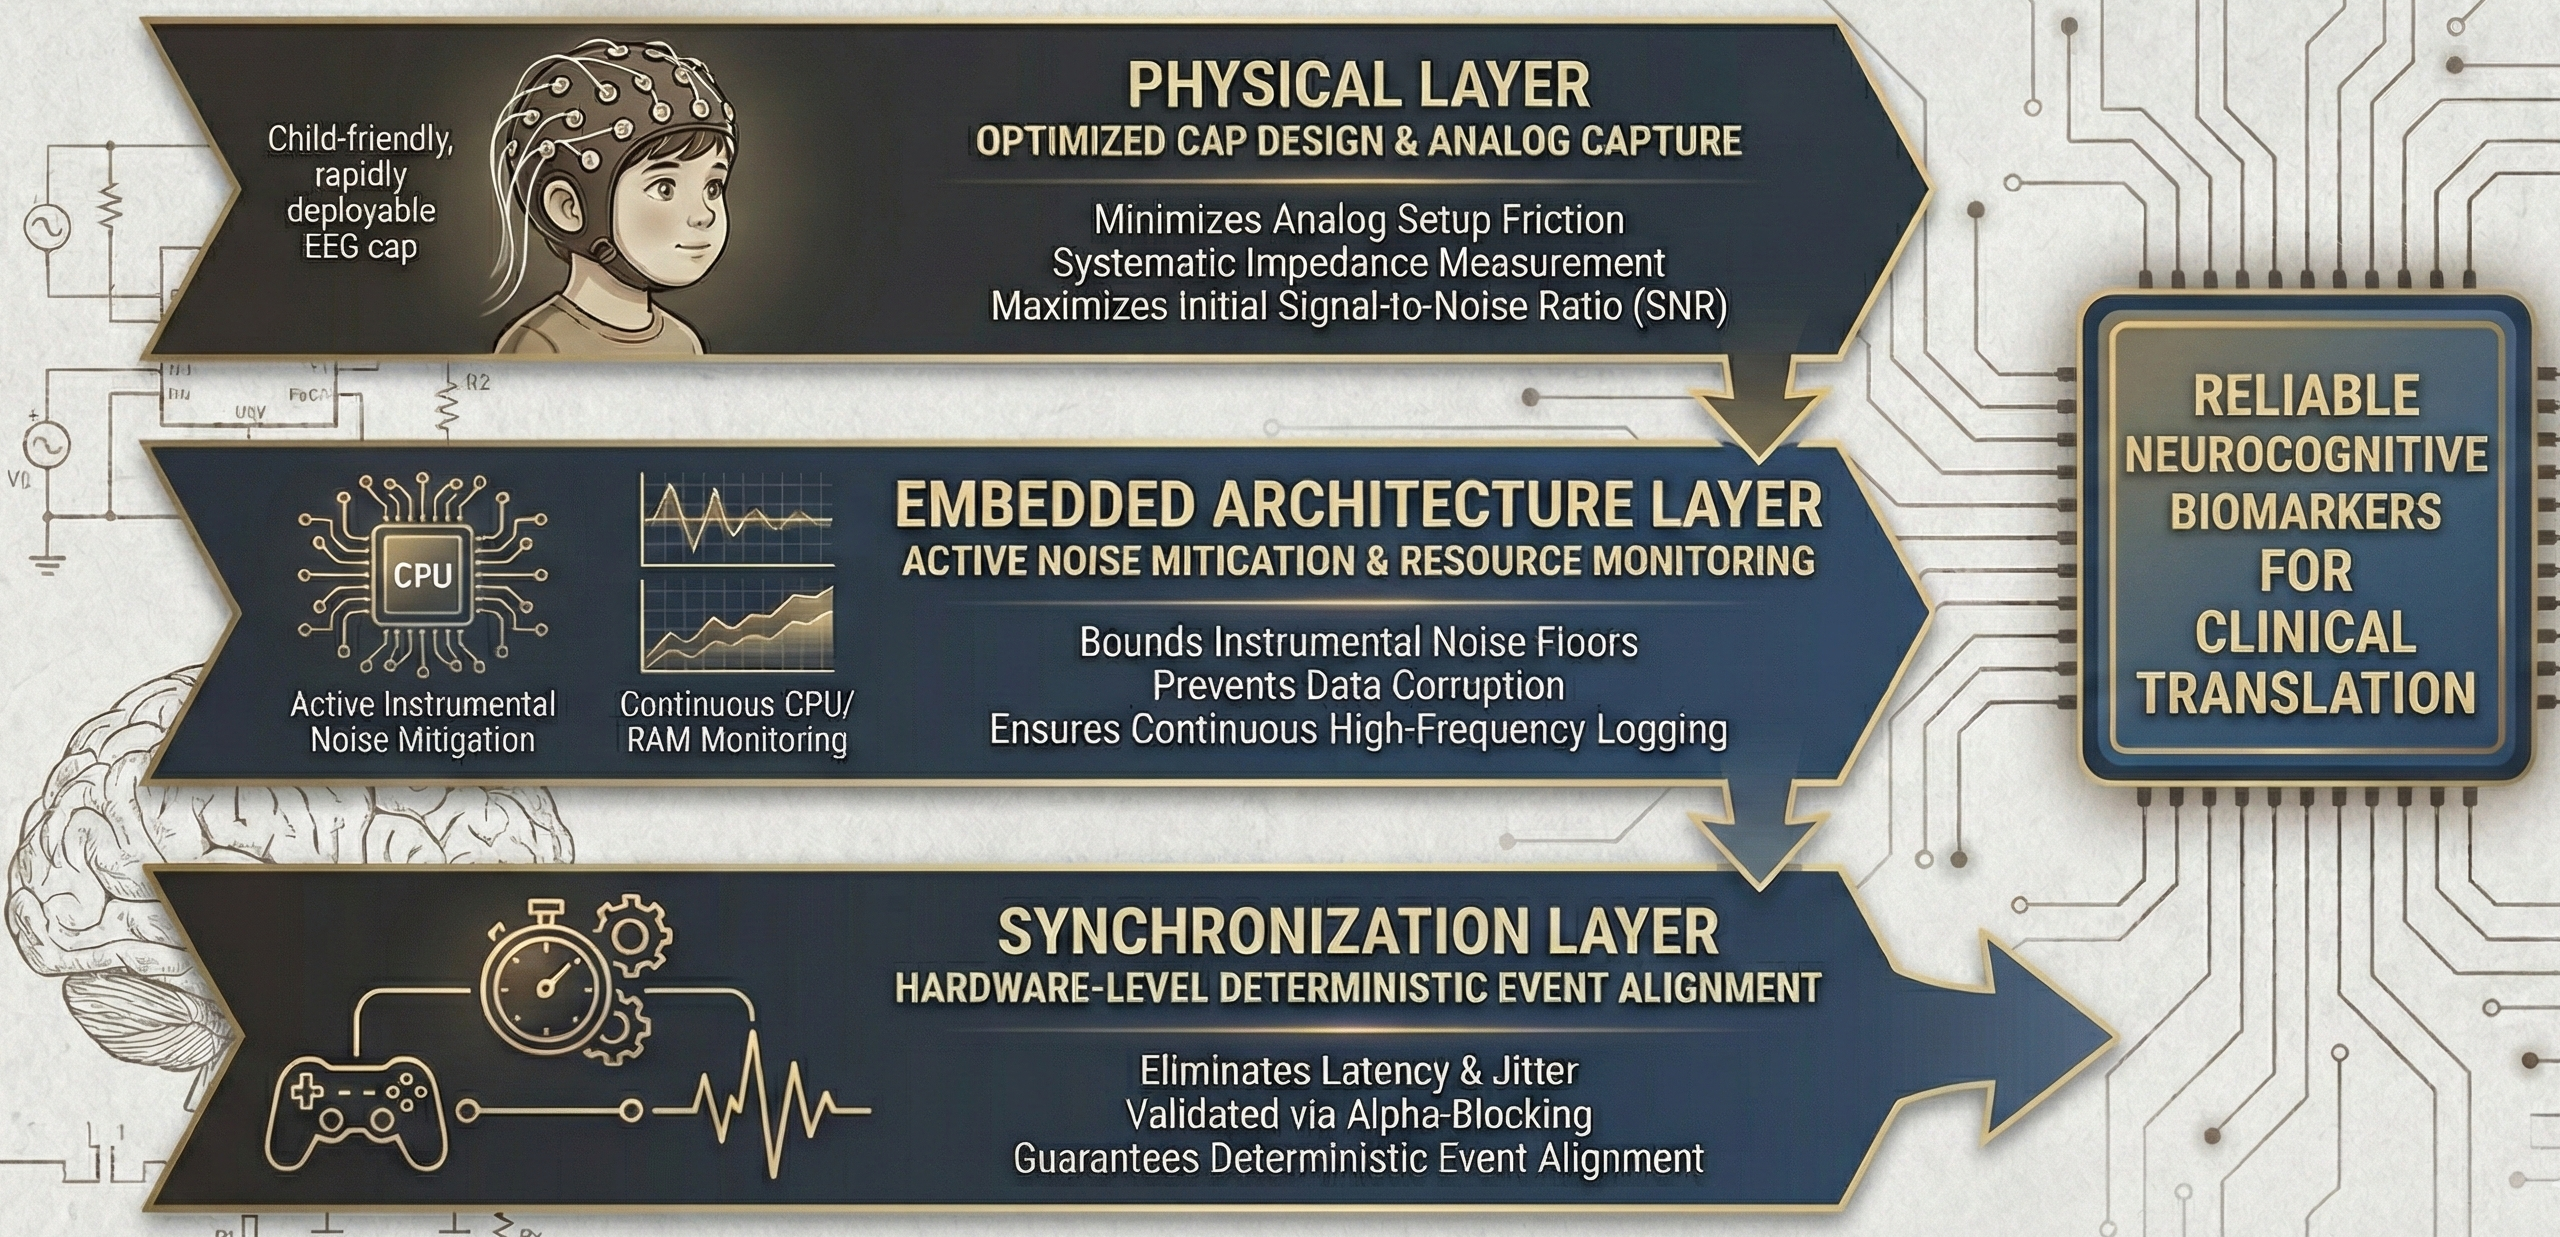
\includegraphics[width=0.8\textwidth]{Cap_1/Figures/contributions.png}
    \caption{These three core contributions form a sequential, interdependent architecture designed to secure neurocognitive data validity. The architecture begins at the \textit{Physical Layer} to secure a pristine baseline signal, passes to the \textit{Embedded Architecture Layer} for noise mitigation and resource management, and concludes in the \textit{Synchronization Layer} to guarantee deterministic event alignment.}
    \label{fig:contributions}
\end{figure}

These core contributions form a sequential, interdependent architecture designed to secure neurocognitive data validity. As illustrated in Figure \ref{fig:contributions}, only when all three sequential layers operate without failure can clinically valid Event-Related Potentials (\glspl{ERP}) be extracted for accurate \gls{ADHD} assessment.

\subsection{Optimized Physical Interface and Analog Capture}

A qualified tool for clinical neurocognitive assessments must overcome physical deployment barriers, especially when dealing with pediatric patients. The architecture begins at the physical layer, where minimizing analog setup friction is required to secure a pristine baseline signal.

Bearing this in mind, we propose a novel, rapidly deployable \gls{EEG} cap design and a systematic electrode-skin impedance measurement protocol. This development overcomes physical barriers and maximizes the initial signal-to-noise ratio (\gls{SNR}), ensuring high-fidelity analog input for the subsequent acquisition stages.

\subsection{Robust Embedded Acquisition Architecture}

The continuous, high-frequency logging of neurophysiological data is highly susceptible to instrumental noise and computational bottlenecks, which can lead to data loss or corruption during continuous assessments.

To mitigate these issues, this work presents the design and implementation of a robust \gls{EEG} acquisition system. This embedded architecture features active instrumental noise mitigation to bound noise floors, alongside continuous system-level resource monitoring (CPU and RAM) to prevent data loss. This layer ensures that the high-fidelity analog input is properly digitized and managed without corruption.

\subsection{Hardware-Level Temporal Synchronization}

The effectiveness of cognitive assessments heavily depends on the system's ability to precisely align acquired physiological signals with external stimuli, requiring low latency and minimal jitter.

To achieve this, we developed a deterministic event-alignment framework that eliminates unpredictable communication latency and jitter. This synchronization layer processes the clean data stream, hardware-locking it to external game stimuli. This approach has been validated through rigorous end-to-end stress testing and physiological alpha-blocking assessments, definitively securing the clinical validity of \glspl{ERP}.

\section{Thesis structure}
\label{sec:thesis_structure}

To detail the design, implementation, and empirical validation of these proposed contributions, the remainder of this thesis is structured as follows: Chapter 2 (\textit{Theoretical Framework}) introduces the fundamental concepts underlying continuous \gls{EEG} monitoring, the electrophysiological manifestations of \gls{ADHD}, mixed-signal embedded hardware design, and principles of data synchronization. Chapter 3 (\textit{Hardware Architecture}) details the methodology behind the physical \gls{EEG} cap, the analog front-end components, and the digital processing unit, while also presenting initial empirical validations such as impedance characterization and embedded system stress testing. Chapter 4 (\textit{Firmware Synchronization}) presents the temporal synchronization architecture, describing the firmware and software methods employed, and covering empirical validations like latency, jitter, multimodal stress tests, and physiological alpha-blocking. Finally, Chapter 5 (\textit{Final Remarks}) summarizes the research findings, evaluates the performance against objectives, details academic contributions, and outlines directions for future improvements.

\chapter{Theoretical Framework}
\label{ch:theoretical_framework}

The development of the MONEEE system is grounded in the convergence of neurophysiological principles, precision electronic engineering, and computer science. This section systematizes the critical concepts required for the device's implementation, addressing the stochastic nature of biological signals, the low-noise acquisition architecture, and the challenges inherent to temporal synchronization in heterogeneous digital systems.

\section{Neurophysiology and Event-Related Potentials (ERPs)}
\label{sec:neurophysiology}

Electroencephalography (EEG) constitutes a non-invasive technique for recording cerebral bioelectric activity via transducers arranged on the scalp. While continuous EEG analysis allows for the monitoring of basal brain states—such as wakefulness, sleep, or convulsive pathologies—cognitive neuroscience research requires isolating specific neuronal responses associated with sensory, motor, or cognitive stimuli. These voltage fluctuations, known as Event-Related Potentials (ERPs), represent the synchronized activity of pyramidal neuronal populations in response to information processing.

\begin{figure}[ht]
    \centering
    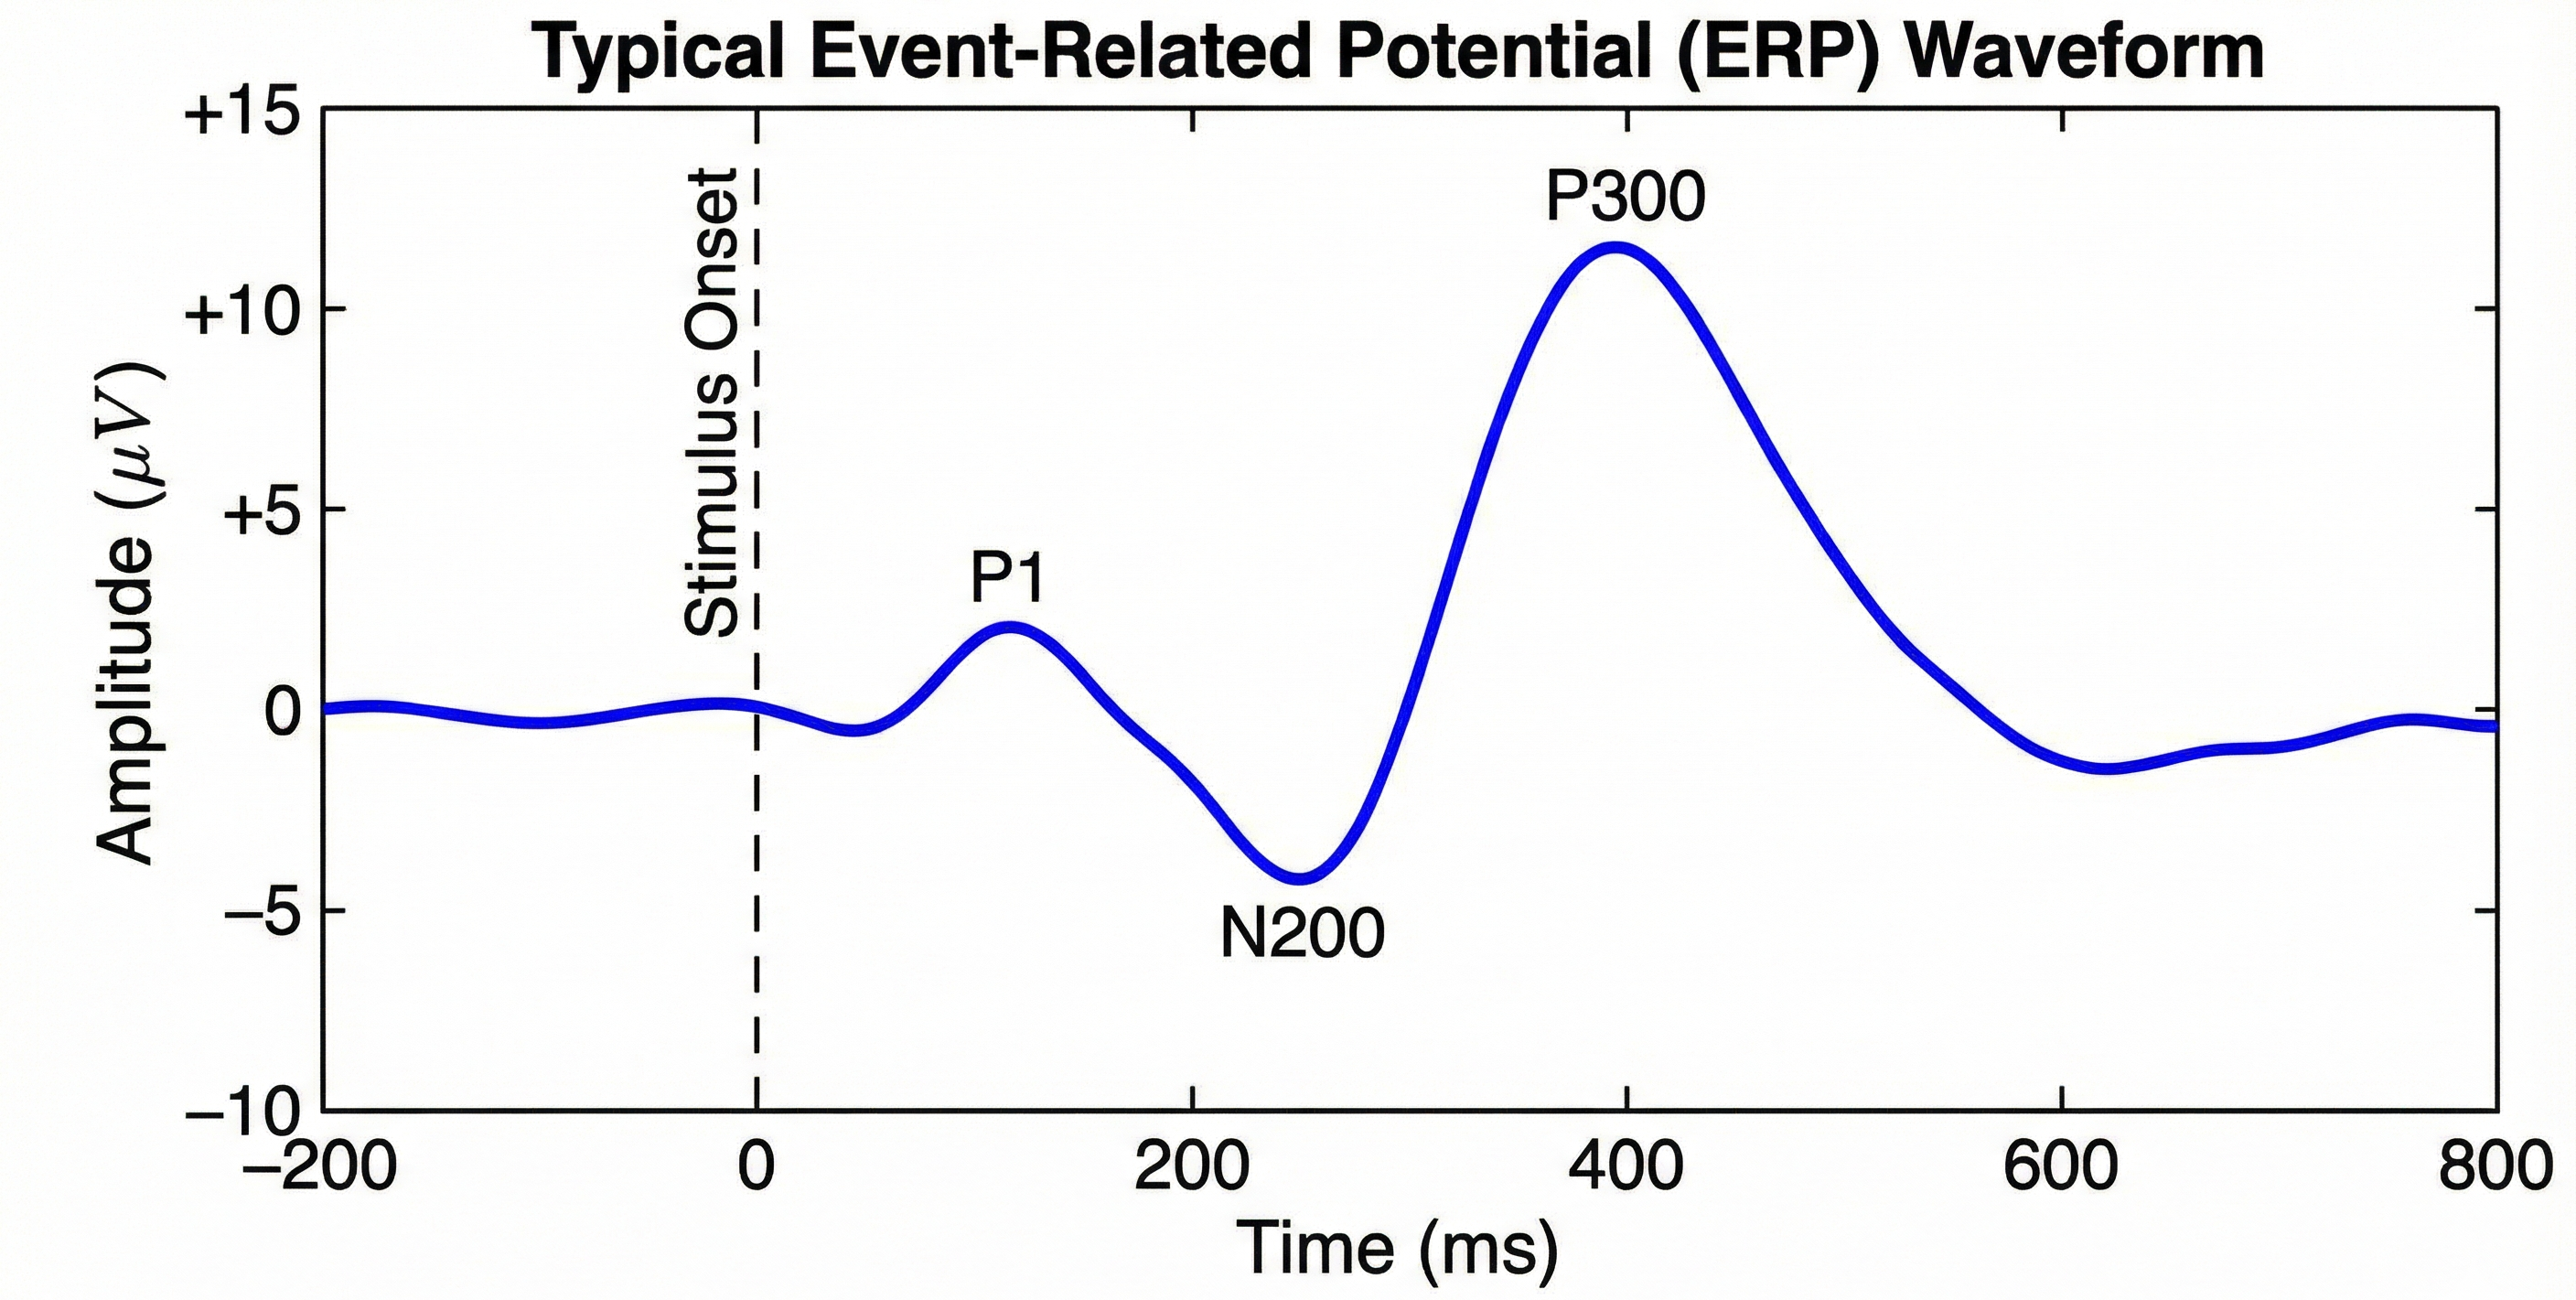
\includegraphics[width=0.8\textwidth]{Cap_2/Figure/p300_waveform.png}
    \caption{Characteristic morphology of an Event-Related Potential (ERP), highlighting exogenous and endogenous components such as the N200 and P300.}
    \label{fig:p300_waveform}
\end{figure}

Within the complex morphology of ERPs, two endogenous components are of particular interest for neurocognitive evaluation and the implementation of serious games in the context of this project. The first is the N200 (or N2) component, a negative deflection that reaches its maximum amplitude between 200 and 350 ms post-stimulus. This component is functionally linked to executive control, specifically in mismatch detection processes and the inhibition of motor responses. The second component, the P300 (or P3b), manifests as a prominent positive deflection with a latency of 300 to 600 ms. Its amplitude is modulated by the allocation of attentional resources and the updating of working memory, being particularly sensitive to stimulus improbability (the \textit{oddball} paradigm). Due to these characteristics, the P300 is consolidated as a robust biomarker for quantifying cognitive load and attentional deficits.

The detection of these components presents a significant challenge in signal processing due to their low signal-to-noise ratio (SNR). ERPs possess typical amplitudes in the range of $1\mu V$ to $20\mu V$, frequently remaining masked by background EEG activity, the magnitude of which oscillates between $50\mu V$ and $100\mu V$. To extract the signal of interest, the technique of coherent signal averaging is employed. Assuming that background noise is a stochastic process with zero mean and is uncorrelated with the stimulus, by averaging $N$ trials, the noise amplitude decreases in proportion to $1/\sqrt{N}$, while the ERP signal remains constant.

However, the validity of this technique depends strictly on temporal stability. Variability in the synchronization marker's latency, a phenomenon termed \textit{jitter}, introduces systematic errors in the resulting average. Mathematically, if the trigger latency follows a normal distribution with standard deviation $\sigma_t$, the averaging process acts as a low-pass filter on the original waveform, attenuating high-frequency components and distorting peak amplitude. A jitter greater than 10 ms ($\sigma_t > 10$ ms) is sufficient to degrade the morphology of the N200 component, compromising the diagnostic utility of the data. Consequently, the MONEEE system must guarantee strict real-time (\textit{hard real-time}) synchronization to preserve the spectral and temporal integrity of the biomarkers.

\section{Hardware Architecture for Signal Acquisition}
\label{sec:hardware}

The fidelity in the digitization of biopotentials is determined by the topology of the Analog Front-End (AFE). The proposed system integrates the Texas Instruments ADS1299 integrated circuit, an analog-to-digital converter (ADC) designed specifically for biomedical instrumentation, which implements a Delta-Sigma ($\Delta\Sigma$) modulation architecture.

Unlike the Successive Approximation Register (SAR) converters common in general-purpose microcontrollers, the $\Delta\Sigma$ architecture offers superior advantages in terms of dynamic range and noise rejection through two main mechanisms: oversampling and noise shaping. The device samples the input signal at a modulation frequency ($f_{mod}$) significantly higher than the Nyquist rate, distributing quantization noise power over a wider spectrum. Subsequently, the modulator shifts this noise toward high frequencies, outside the biological band of interest (0--100 Hz), allowing a digital decimation filter to eliminate it effectively while reducing the data rate to the output frequency configured by the user.

\begin{figure}[ht]
    \centering
    \includegraphics[width=0.8\textwidth]{Cap_2/Figure/delta_sigma_block.png}
    \caption{Simplified functional scheme of the modulation and filtering stage in a Delta-Sigma architecture ADC.}
    \label{fig:delta_sigma}
\end{figure}

A critical aspect for functional connectivity and EEG coherence analysis is sampling simultaneity. In traditional multiplexed systems, a single ADC core switches sequentially between channels, introducing a systematic phase delay ($t_{skew}$) between electrodes. The ADS1299 mitigates this problem by incorporating independent $\Delta\Sigma$ modulators for each of its 8 channels, guaranteeing a virtually null $t_{skew}$ and preserving the real phase relationship between different cortical regions.

To manage data flow without sacrificing temporal determinism, the MONEEE system design adopts a heterogeneous computing architecture that decouples acquisition from high-level processing. This structure is composed of a Microcontroller Unit (MCU), such as the TM4C1294, and a Microprocessor Unit (MPU), based on embedded Linux. The MCU operates under real-time constraints (either on \textit{bare-metal} or with a lightweight RTOS), reacting to ADC hardware interrupts (\texttt{DRDY}) on microsecond scales to capture and timestamp samples, preventing FIFO buffer overflows. Meanwhile, the MPU manages computationally intensive and non-deterministic tasks, such as the TCP/IP protocol stack and file system storage. This division of responsibilities isolates bio-signal acquisition from the variable latencies introduced by the Linux kernel scheduler, ensuring data temporal integrity.

\section{Digital Synchronization Protocols}
\label{sec:sync_protocols}

Precise synchronization between the physiological recording and events generated by the stimulation software (video game) constitutes the central technical challenge of this research. The selection of the synchronization method implies a trade-off between temporal precision, implementation complexity, and intrusion into the user experience. Table \ref{tab:sync_methods} summarizes the characteristics of the predominant approaches.

\begin{table}[ht]
    \centering
    \caption{Comparative analysis of synchronization methods for BCI systems.}
    \label{tab:sync_methods}
    \begin{tabular}{p{3cm} p{5cm} p{2.5cm} p{3.5cm}}
        \toprule
        \textbf{Method} & \textbf{Mechanism} & \textbf{Precision} & \textbf{Implementation} \\
        \midrule
        Optical (Photodiode) & Physical detection of screen luminance changes by an external sensor. & High ($<1$ ms) & High (Additional hardware required). \\
        Network (LSL) & Synchronization via local network protocol and software jitter correction. & Medium ($<5$ ms) & Low (Software only). \\
        Hardware Trigger (TTL) & Direct electrical signal from Parallel/USB port to the ADC. & Very High ($<1$ ms) & Medium (Requires specific interfaces). \\
        \bottomrule
    \end{tabular}
\end{table}

There are contrasting approaches to addressing this problem. Optical synchronization, based on photodiodes attached to the monitor, is considered the ``gold standard'' for validation, as it detects the physical change of pixels, bypassing software, operating system, and GPU rendering latencies. However, its requirement for external hardware limits its viability in massive clinical deployments. As a scalable alternative, the \textit{Lab Streaming Layer} (LSL) protocol offers a middleware solution that unifies disparate data streams by assigning timestamps referenced to a common clock and drift correction algorithms. While LSL simplifies integration, its final accuracy remains dependent on local network stability and the game engine's ability to report the event time accurately.

In the context of the MONEEE system's physical interface, the USB bus introduces non-trivial latency considerations, especially for the transmission of marking commands (\textit{soft-triggers}) from the PC to the amplifier. As a host-controlled bus utilizing polling, data transfer is discretized into frame intervals (1 ms in \textit{Full Speed}) or microframes ($125 \mu s$ in \textit{High Speed}). Additionally, the use of the CDC (\textit{Communication Device Class}) to emulate serial ports implies that data traverses the operating system driver stack, where it may be stored in intermediate buffers to optimize global system performance. This behavior introduces variable and unpredictable latencies of several milliseconds between the logical generation of the event in the game and its physical arrival at the USB bus, which is incompatible with the precision requirements for high-frequency ERP component analysis.

To address the latency indeterminacy introduced by the USB stack and OS buffering, the MONEEE system implements a \textit{hardware-embedded synchronization protocol} that couples synchronization logic directly to the biological sample at the firmware level. Unlike architectures that transmit event markers and EEG data through separate logical channels, MONEEE adopts a specific hexadecimal frame structure where the initial three bytes are strictly reserved for control data, thereby eliminating the need for post-hoc timestamp realignment.

In this encoding scheme, the first byte acts as a binary Event Flag ($B_{0}$), explicitly indicating the presence of a synchronization trigger with a value of \texttt{1} or a resting state with \texttt{0}, while the second byte ($B_{1}$) designates the Event Type, carrying the specific code required to classify the nature of the stimulus (e.g., distinguishing between target and standard inputs). This metadata is immediately followed by the third byte ($B_{2}$), which serves as a static Start-of-Frame delimiter to identify the beginning of the physiological data payload. By packaging the event markers and the EEG signal within this same atomic transmission unit, the system transforms the synchronization problem into a data parsing task, ensuring that the relative phase relationship is preserved regardless of the jitter introduced by the USB communication or the operating system scheduler.

% --- Place this immediately after the text about the frame structure ---


\chapter{Hardware Architecture (The MONEEE System)}
\label{ch:hardware_architecture}

The engineering design of the MONEEE system addresses the critical need to capture low-amplitude biopotentials with a high signal-to-noise ratio, while simultaneously guaranteeing low-latency synchronization with external events. To satisfy these requirements, a heterogeneous embedded computing architecture has been implemented, physically decoupling the real-time acquisition domain from the high-level computational domain. This separation allows each subsystem to be optimized for its specific function: signal integrity and determinism for acquisition, and performance and connectivity for processing.

\section{System Topology and Data Flow}
\label{sec:system_overview}

The device operates under an \textit{edge-computing} paradigm, dedicating its resources exclusively to EEG signal management. The architecture establishes a strictly unidirectional data flow from the patient toward the processing unit, designed to minimize transport latency. The signal chain is formally modeled by the following transduction and transmission sequence:

\begin{equation}
    \text{Electrodes} \xrightarrow{\text{Analog}} \text{ADS1299} \xrightarrow{\text{SPI}} \text{TM4C1294} \xrightarrow{\text{SPI}} \text{RPi CM4}
\end{equation}

As illustrated in Figure \ref{fig:block_diagram}, the hardware is structured into three differentiated functional zones: the Analog Front-End (AFE), the Real-Time Core, and the Compute Core. This segmentation is not merely logical but physical, employing isolation barriers to protect the integrity of physiological measurements.

\begin{figure}[htbp]
    \centering
    \includegraphics[width=0.85\textwidth]{Cap_3/Figure/DBP.png}
    \caption{Block diagram of the MONEEE architecture, evidencing the segregation between the deterministic acquisition (MCU) and high-level processing (MPU) domains.}
    \label{fig:block_diagram}
\end{figure}

For this project, we have established the MONEEE system as a robust electronic design aligned with acquisition systems in its segment. The designs presented in Figures \ref{fig:modulo_eeg}, \ref{fig:filtros_acople}, \ref{fig:modulo_comunicacion}, \ref{fig:led_head}, \ref{fig:board_ads}, and \ref{fig:cpu} illustrate our proposal for an EEG signal acquisition board, conceived to significantly improve the capacity of real-time BCI systems, overcoming current challenges and contributing to the advancement of technology in this field.

\subsection{Electronic Design}
\label{subsec:electronic_design}

The following schematic designs constitute the complete electronic architecture of the MONEEE system, divided by their primary functions.

%=======================================

\begin{figure}[htbp]
    \centering
    \includegraphics[width=0.65\linewidth]{Cap_3/Figure/ModuloEEG.png}
    \caption{Schematic design for the module responsible for acquiring EEG signals.}
    \label{fig:modulo_eeg}
\end{figure}

%====================================

\begin{figure}[htbp]
    \centering
    \includegraphics[width=0.65\linewidth]{Cap_3/Figure/Filtros electrodos.png}
    \caption{Schematic design of coupling filters.}
    \label{fig:filtros_acople}
\end{figure}

%====================================

\begin{figure}[htbp]
    \centering
    \includegraphics[width=0.65\linewidth]{Cap_3/Figure/Modulo comunicacion.png}
    \caption{Schematic design of the module responsible for communicating the collected data to another device or to the cloud.}
    \label{fig:modulo_comunicacion}
\end{figure}

%====================================

\begin{figure}[htbp]
    \centering
    \includegraphics[width=0.65\linewidth]{Cap_3/Figure/Led_head.png}
    \caption{Module for impedance visualization of the electrodes.}
    \label{fig:led_head}
\end{figure}

%====================================

\begin{figure}[htbp]
    \centering
    \includegraphics[width=0.65\linewidth]{Cap_3/Figure/Board_ADS.png}
    \caption{Connection between the different ADS1299 acquisition modules.}
    \label{fig:board_ads}
\end{figure}

%====================================

\begin{figure}[htbp]
    \centering
    \includegraphics[width=0.65\linewidth]{Cap_3/Figure/MONEEE_CPU.png}
    \caption{Motherboard for microcontroller and microprocessor.}
    \label{fig:cpu}
\end{figure}

\section{Analog Front-End (AFE) and Biomedical Interface}
\label{sec:analog_front_end}

The interface between the biological medium and the digital system is realized via the Texas Instruments ADS1299 integrated circuit. This component, a 24-bit analog-to-digital converter (ADC) with 8 simultaneous channels, has been specifically configured to optimize surface electroencephalography capture.

To maximize effective resolution on signals typically oscillating between $10$ and $100 \mu V$, the internal Programmable Gain Amplifier (PGA) is set to a gain of $24V/V$. Likewise, the sampling rate is fixed at 250 SPS or 500 SPS. This frequency provides a bandwidth that exceeds Nyquist requirements for the spectral components of interest (P300 and N200, generally located below 30 Hz), while allowing for the advantages of oversampling to reduce the noise floor. The input multiplexer is maintained in NORMAL mode for electrode acquisition, preserving the capability to internally switch toward test signals for self-calibration routines.

The suppression of electromagnetic interference, primarily 50/60 Hz mains noise, is managed through an active Driven Right Leg (DRL) topology. Unlike a passive ground reference, the ADS1299's \textit{Bias Drive} circuit monitors the common-mode voltage present at the detection electrodes. This signal is inverted, amplified, and reinjected into the patient's body through the reference electrode. This negative feedback loop actively cancels interference, raising the Common-Mode Rejection Ratio (CMRR) to levels exceeding $110$ dB, which is indispensable for unshielded clinical environments.

Finally, signal integrity is ensured through rigorous power management. The AFE is powered by a dedicated Li-Po battery and regulated by a PMIC (Power Management Integrated Circuit). The analog power domain ($AVDD$) is isolated from digital rails via Low-Dropout Regulators (LDOs) with high Power Supply Rejection Ratio (PSRR). This strategy prevents high-frequency switching noise, inherent to CPU operation in the compute module, from capacitively coupling to the amplifier input stages.

\section{The Digital Core: Heterogeneous Processing}
\label{sec:digital_core}

The digital architecture implements a shared responsibility model, distributing the computational load between a real-time microcontroller and an application microprocessor.

The Real-Time Unit, driven by a Texas Instruments TM4C1294 (ARM Cortex-M4F), serves as the acquisition system master. Operating in a \textit{bare-metal} environment or under a lightweight real-time operating system, the TM4C ensures deterministic performance. Its primary role is to immediately service the \texttt{DRDY} (Data Ready) hardware interrupt generated by the ADC, guaranteeing lossless sample capture. Moreover, the integration of a Floating-Point Unit (FPU) allows for the application of in-situ digital pre-processing—such as notch filtering or scaling—without impacting interrupt service latency. At this critical juncture, each sample is assigned a hardware \textit{timestamp}, achieving microsecond-level temporal precision.

Data is subsequently routed to the Compute Unit, implemented via a Raspberry Pi Compute Module 4 (CM4). Executing a full Linux operating system, this module is tasked with higher-level organizational roles: mass storage management, deployment of the \textit{Lab Streaming Layer} (LSL) gateway, and telemetric transmission over Wi-Fi. The CM4 aggregates the continuous data stream transmitted by the microcontroller and packages it into standardized structures suitable for consumption by the interactive game software.

Communication between the real-time and compute cores depends on a high-speed serial interface (UART operating at $>921600$ baud or SPI). To guarantee patient safety and preserve signal integrity, this digital link utilizes galvanic isolation (e.g., standard digital isolators like the ISO77xx series). This configuration prevents the formation of ground loops between the battery-powered floating acquisition stage and any peripheral connected to the electrical grid. The communication protocol relies on lightweight binary frames that encapsulate the 24-bit data alongside their corresponding timestamps; these frames are authenticated by a Cyclic Redundancy Check (CRC) to verify transmission integrity.


\section{Event Synchronization Interface (USB-C)}
\label{sec:event_interface}

Synchronization with the stimulation platform (e.g., a tablet) is physically facilitated by a USB Type-C port. Managed by the system's USB controller, this interface enables the reception of "event markers" generated by the game software at the precise instance of stimulus presentation. Because standard commercial devices introduce considerable electrical noise—primarily due to internal DC-DC converters—the MONEEE framework employs total isolation of the USB bus. The differential data lines ($D+/D-$) are routed through a specialized isolation integrated circuit (e.g., the ADuM3160), actively eliminating galvanic continuity.

To handle the transmission of these synchronization markers from the software side, the system deploys \texttt{MoneLib}, a custom library that bridges the Unity-based simulation environment with the embedded hardware. Compiling as a native Android plugin (\texttt{.aar}), this library empowers the game engine to communicate directly with the USB Host subsystem of the tablet. The associated software architecture strictly mandates an Android device running version 12 (Snow Cone) or later with robust USB-C Host support in order to initialize the communication driver properly.

The underlying communication protocol is streamlined for low latency by encoding game events—such as player selections or application states—into lightweight hexadecimal values transmitted over USB. For example, marking an "O" transmits \texttt{0x00}, asserting an "X" transmits \texttt{0x01}, and initiating a system restart triggers \texttt{0xFF}. To preserve signal integrity and preclude the saturation of the USB channel, the protocol enforces a mandatory safety interval of exactly one millisecond between consecutive event transmissions.

Through this systemic interface, the "Serious Game" acts as a precision stimulation trigger. Whenever a user interacts with the application, the \texttt{MoneLibrary.SendUsbData} routine is immediately invoked, securely dispatching the corresponding integer to the downstream microcontroller. The incoming hardware event is subsequently captured and precisely timestamped by the embedded USB peripheral, ensuring that the subjective cognitive task tightly correlates with the objective physiological recording, thus enabling robust post-hoc analysis.

\begin{figure}[H]
    \centering
    \begin{tikzpicture}[
            node distance=3.8cm, % Increased distance to prevent vertical overlapping
            auto,
            block/.style={
                    rectangle,
                    draw=black,
                    thick,
                    fill=blue!5,
                    text width=16em, % Widened to fit "Hardware Abstraction Layer" on one line
                    align=center,
                    rounded corners,
                    minimum height=4em
                },
            cloud/.style={
                    draw=black,
                    thick,
                    ellipse,
                    fill=green!5,
                    minimum height=3em,
                    text width=12em,
                    align=center
                },
            arrow/.style={
                    thick,
                    ->,
                    >=stealth
                }
        ]

        % Nodes
        \node [cloud] (user) {User Interaction \\ (Touch Event)};

        \node [block, below of=user, node distance=3cm] (unity) {
            \textbf{Unity Game Engine} \\
            \textit{C\# Script Layer} \\
            \texttt{OnCellClick()}
        };

        \node [block, below of=unity] (monelib) {
            \textbf{MoneLib Middleware} \\
            \textit{Android Native Plugin (.aar)} \\
            \texttt{SendUsbData(sbyte)}
        };

        \node [block, below of=monelib] (usb) {
            \textbf{Android USB Host} \\
            \textit{Hardware Abstraction Layer} \\
            (USB-C Controller)
        };

        \node [block, below of=usb, fill=orange!10, dashed] (mcu) {
            \textbf{MONEEE MCU} \\
            \textit{External Embedded System} \\
            (Timestamp Generation)
        };

        % Edges and Labels (using xshift to separate left/right labels)
        \draw [arrow] (user) -- node {Trigger} (unity);

        \draw [arrow] (unity) -- node[right, xshift=0.2cm] {Call Library} node[left, xshift=-0.2cm] {\texttt{0x00} / \texttt{0x01}} (monelib);

        \draw [arrow] (monelib) -- node {JNI Bridge} (usb);

        \draw [arrow] (usb) -- node[right, xshift=0.2cm] {Physical Trans.} node[left, xshift=-0.2cm] {USB D+/D-} (mcu);

        % Protocol Legend Box
        \node [draw=black, thin, align=left, right of=monelib, node distance=7.5cm, text width=4.5cm] (legend) {
            \textbf{Protocol Map:} \\
            \texttt{0x00}: Mark 'O' \\
            \texttt{0x01}: Mark 'X' \\
            \texttt{0xFF}: Restart \\
            \textit{Interval:} $>1$ms
        };

        \draw [dashed, gray] (monelib) -- (legend);

    \end{tikzpicture}
    \caption{Data flow diagram of the Event Synchronization Interface. The high-level interaction within Unity is transduced into a hexadecimal marker by the MoneLib middleware and transmitted via the USB isolation barrier to the MONEEE acquisition core.}
    \label{fig:usb_sync_flow}
\end{figure}

\subsection{Desktop Application: MONEEE Visualizer}
\label{subsec:moneee_visualizer}

To complement the embedded hardware architecture and provide a comprehensive interface for data monitoring, a dedicated EEG signal analytical suite known as the MONEEE Visualizer was developed. This application facilitates the real-time observation and analysis of the acquired electroencephalographic data streams. By employing this tool, researchers can actively monitor signal quality, verify electrode contacts, and validate overall system performance iteratively during experimental paradigms. The graphical user interface of the MONEEE visualizer is documented in Figure \ref{fig:moneee_visualizer}.

\begin{figure}[H]
    \centering
    \includegraphics[width=0.8\textwidth]{Cap_3/Figure/MONEEE_visualizer.png}
    \caption{Graphical user interface of the MONEEE visualizer.}
    \label{fig:moneee_visualizer}
\end{figure}

\section{Hardware Validation Strategy}
\label{sec:hardware_validation}

To rigorously demonstrate that the MONEEE system satisfies the stringent prerequisites for clinical-grade EEG acquisition, an initial sequence of hardware validation tests has been established. These structured protocols are purposefully designed to verify the fidelity of the physical interface and characterize the baseline analog performance of the system prior to any digital integration or filtering.

\subsection{Use and Impedance Measurement Test of the New Cap}
Maintaining optimal electrode-skin contact is fundamental for acquiring high-quality EEG recordings. This test systematically evaluates the usability and anatomical congruence of the custom EEG cap, verifying the application of consistent mechanical pressure across the scalp. Consequently, the electrical impedance of the electrode-skin interface is actively quantified utilizing the integrated lead-off detection circuitry of the ADS1299. This subsystem injects a calibrated AC or DC excitation current directly into the electrodes, allowing the MCU to derive and monitor contact quality in real time. The resulting impedance status is visually communicated to the operator via the dedicated impedance visualization module (Figure \ref{fig:led_head}), facilitating rapid, localized adjustments prior to commencing an experimental paradigm. A visual representation of this impedance checking sequence is provided in Figure \ref{fig:check_impedance}.

\begin{figure}[H]
    \centering
    \includegraphics[width=1.0\textwidth]{Cap_3/Figure/check_impedance.png}
    \caption{Visualization of the impedance checking process.}
    \label{fig:check_impedance}
\end{figure}

\subsection{Instrumental Noise Characterization (Noise Floor)}
To validate the capacity of the Analog Front-End to accurately digitize microvolt-level physiological signals, an instrumental noise baseline characterization is performed. During this evaluation, the input channels of the ADS1299 are internally shorted to ground, effectively quantifying the intrinsic electronic noise generated by the internal amplifiers and the ADC, independently of ambient interference or skin impedance loading. The resulting input-referred noise floor is analyzed to ensure that both the peak-to-peak and root-mean-square (RMS) noise magnitudes comply with the sub-microvolt specifications necessary for the reliable extraction of subtle Event-Related Potentials (ERPs). It is important to note that the graph presented in Figure \ref{fig:noise_plot} exhibits elevated values because the test was conducted in an environment with high external noise caused by interference from adjacent equipment.

\begin{figure}[H]
    \centering
    \includegraphics[width=0.8\textwidth]{Cap_3/Figure/noise_plot.pdf}
    \caption{Instrumental noise characterization with the ADS1299 inputs internally short-circuited. The elevated values observed are indicative of interference generated by adjacent external equipment during the test.}
    \label{fig:noise_plot}
\end{figure}
\chapter{Firmware Architecture and Temporal Synchronization Strategy}
\label{ch:firmware_sync}

This section delves into the embedded computational logic governing the MONEEE hardware and its interface with the simulation environment. It describes the central methodological contribution of this development: a hardware-level event injection mechanism designed to mitigate the stochastic latency inherent to general-purpose operating systems, thereby achieving precise synchronization between physiological data and game stimuli at the microcontroller (MCU) level.

\section{Deterministic Firmware Design on the TM4C1294}
\label{sec:tm4c_firmware}

The firmware resident on the Texas Instruments TM4C1294 microcontroller has been structured under a \textit{bare-metal} paradigm (dispensing with a complex operating system) to guarantee strictly deterministic behavior. The software architecture is event-driven, establishing an execution hierarchy where data acquisition holds maximum priority, subordinating any communication or maintenance tasks.

The synchronization engine depends on the precise management of the \texttt{DRDY} (Data Ready) interrupt signal generated by the ADS1299 converter. This signal activates the capture logic at the programmed sampling frequency (e.g., 250 Hz, corresponding to a 4 ms period).

\begin{figure}[h!]
    \centering
    \includegraphics[width=0.8\textwidth]{Cap_4/Figure/isr_flowchart.png}
    \caption{Flowchart of the Interrupt Service Routine (ISR) associated with the Data Ready signal (DRDY).}
    \label{fig:isr_flowchart}
\end{figure}

The sequence of operations within the Interrupt Service Routine (ISR), as illustrated in Figure \ref{fig:isr_flowchart}, is critical for maintaining the system's phase coherence. Upon detection of the falling edge of the \texttt{DRDY} signal, the microcontroller activates the \textit{Chip Select} (\texttt{CS}) line of the SPI bus and initiates a Direct Memory Access (DMA) transfer. This mechanism allows for the automatic reading of 24 bytes of data (8 channels of 24 bits plus status bits) without CPU intervention, which is reserved for managing storage in a circular buffer and verifying event flags.

\subsection{Hardware Event Injection Strategy (MCU-to-Aggregator Egress Protocol)}
To resolve the problem of temporal desynchronization, the system design dispenses with PC or Raspberry Pi clocks for event \textit{timestamping}. Instead, a direct injection strategy into the data frame is implemented. This protocol governs the egress data flow from the microcontroller to the aggregation node.

The operation of this mechanism is based on the immediate reception of commands. When the stimulation software (Game) generates a visual event, it transmits an 8-bit hexadecimal code (e.g., \texttt{0x0A}) via the USB-C interface to the TM4C. The arrival of this byte triggers a high-priority interrupt in the MCU, which immediately stores the value in a volatile register named \texttt{Current\_Event}. During the subsequent ADS1299 sampling cycle (which occurs within an interval of less than 4 ms), the ISR queries this register and concatenates the event code directly to the end of the EEG data packet in progress. In this way, the event marker and the physiological sample become physically linked within the same data structure before being transmitted to the Linux environment. This approach ensures that the relative \textit{jitter} between the stimulus and the biological response is virtually null, bounded only by the temporal resolution of the sampling period.

To formalize this linkage between physiological data and event markers, the system employs a specific hexadecimal frame structure for serial transmission to the aggregation node, as visualized in Figure \ref{fig:moneee_frame_structure}. In this encoding scheme, the initial three bytes are strictly reserved for control data, thereby eliminating the need for post-hoc timestamp realignment. The first byte acts as a binary Event Flag ($B_{0}$), explicitly indicating the presence of a synchronization trigger with a value of \texttt{1} or a resting state with \texttt{0}. The second byte ($B_{1}$) designates the Event Type, carrying the specific code required to classify the nature of the stimulus (e.g., distinguishing between target and standard inputs, populated directly from the \texttt{Current\_Event} register). This metadata is immediately followed by the third byte ($B_{2}$), which serves as a static Start-of-Frame delimiter (\texttt{0xFE}) to identify the beginning of the physiological data payload. By packaging the event markers and the EEG signal within this same atomic transmission unit, the system transforms the synchronization problem into a data parsing task, ensuring that the relative phase relationship is preserved regardless of the jitter introduced by subsequent USB communication or operating system schedulers.

\begin{figure}[ht]
    \centering
    % Define custom colors for clarity
    \definecolor{moneeeSync}{RGB}{255, 100, 100} % Red-ish for sync events
    \definecolor{moneeeSOF}{RGB}{255, 200, 0}   % Yellow-ish for Start of Frame
    \definecolor{moneeeData}{RGB}{100, 200, 100} % Green-ish for payload

    \begin{tikzpicture}[
            font=\sffamily,
            node distance = 0pt,
            start chain = going right,
            byte node/.style = {
                    rectangle,
                    draw=black!80,
                    thick,
                    minimum width=2.2cm,
                    minimum height=1.2cm,
                    outer sep=0pt,
                    align=center,
                    font=\ttfamily\bfseries
                },
            label node/.style = {
                    font=\footnotesize\sffamily,
                    align=center,
                    below=0.3cm
                }
        ]

        % --- Draw the Bytes ---
        % Byte 0: Event Flag
        \node [byte node, on chain, fill=moneeeSync!30] (b0) {0x01};
        % Byte 1: Event Type
        \node [byte node, on chain, fill=moneeeSync!30] (b1) {Type ID};
        % Byte 2: SOF Delimiter
        \node [byte node, on chain, fill=moneeeSOF!30] (b2) {0xFE};
        % Byte 3: Data High
        \node [byte node, on chain, fill=moneeeData!30, right=0.5cm of b2] (d1) {CH1 High};
        % Byte 4: Data Low
        \node [byte node, on chain, fill=moneeeData!30] (d2) {CH1 Low};
        % Continuation dots
        \node [on chain, minimum width=1.5cm, align=center, font=\huge] (dots) {...};
        % Last Byte example
        \node [byte node, on chain, fill=moneeeData!30] (dn) {CHN Low};


        % --- Add Labels below the bytes ---
        \node [label node, below=of b0] {Byte $B_0$\\Event Flag\\(Active=1)};
        \node [label node, below=of b1] {Byte $B_1$\\Event Type\\(Payload)};
        \node [label node, below=of b2] {Byte $B_2$\\Start of Frame\\(Fixed Header)};

        % Group label for EEG data
        \node [label node, below=of d1.south west] (dataLabelStart) {};
        \node [label node, below=of dn.south east] (dataLabelEnd) {};
        \draw [thick, decoration={brace, mirror, raise=0.3cm}, decorate] (d1.south west) -- (dn.south east) node [pos=0.5, below=0.6cm, font=\footnotesize\sffamily] {Physiological Data Payload (EEG Samples)};


        % --- Grouping Backgrounds and Titles ---
        \begin{scope}[on background layer]
            % Sync Header Group
            \node [draw=moneeeSync!80, thick, dashed, fit=(b0) (b2), inner ysep=15pt, inner xsep=5pt, rounded corners, label={[anchor=north, font=\footnotesize\bfseries, text=moneeeSync!80]north:Hardware Synchronization Header (3 Bytes)}] (syncHeader) {};
        \end{scope}

        % --- Transmission Flow Arrow ---
        \draw [-{Latex[length=4mm, width=3mm]}, very thick, gray] ($(b0.west) + (-0.8, 1.5)$) -- node[above, font=\small\bfseries] {Transmission Direction (Serial Stream)} ($(dn.east) + (0.5, 1.5)$);

    \end{tikzpicture}
    \caption{Visual representation of the MONEEE serial data transmission frame. The initial three bytes ($B_0, B_1, B_2$) form a dedicated hardware synchronization prefix attached to every physiological sample, ensuring that event timing is locked to the data stream before transmission to the CM4.}
    \label{fig:moneee_frame_structure}
\end{figure}

\section{Integration Protocol with the Simulation Environment (Tablet-to-MCU Ingress Protocol)}
\label{sec:game_integration}

Interaction with the serious game, developed in the Unity engine, is managed via a custom communication library that acts as an abstraction layer over the tablet's serial API. This library exposes high-level methods, such as \texttt{SendMarker(int code)}, which are invoked by the game logic at the exact instant of stimulus rendering.

To guarantee the integrity of commands transmitted over the USB link and prevent the erroneous interpretation of electromagnetic noise as valid events, a robust binary communication protocol (Ingress Protocol) has been defined for the Stimulus-to-MCU link. The transmission structure consists of 3-byte frames, detailed in Table \ref{tab:protocol}, which is distinct from the 3-byte MCU-to-CM4 egress protocol described in Section \ref{sec:tm4c_firmware}.

\begin{table}[ht]
    \centering
    \caption{Definition of the Serial Event Transmission Protocol.}
    \label{tab:protocol}
    \begin{tabular}{ccc}
        \toprule
        \textbf{Byte 0 (Header)} & \textbf{Byte 1 (Payload)} & \textbf{Byte 2 (Footer)} \\
        \midrule
        Start Marker             & Event Code                & Validation               \\
        \texttt{0xFF}            & \texttt{0x00 - 0xFE}      & \texttt{0xAA}            \\
        \bottomrule
    \end{tabular}
\end{table}

The protocol uses the byte \texttt{0xFF} to signal the start of a transaction, followed by the event identifier (where specific codes denote states such as login, standard stimulus, or \textit{oddball} stimulus). The frame concludes with the byte \texttt{0xAA}, used for integrity validation; any sequence that does not respect this structure is immediately discarded by the TM4C firmware, ensuring high noise immunity.

\section{Processing in the Compute Module (Raspberry Pi CM4)}
\label{sec:rpi_software}

The Raspberry Pi Compute Module 4 plays the role of an aggregation node and data gateway. While strict synchronization is the responsibility of the microcontroller, the CM4 must process the information flow with sufficient efficiency to prevent communication buffer overflows.

To minimize operating system-induced latency, the Linux kernel on the CM4 has been optimized using the \textit{PREEMPT\_RT} patch. This modification transforms Linux into a real-time operating system, allowing execution threads associated with hardware drivers (such as the UART receiver) to preempt standard user-space processes. Additionally, core isolation techniques are employed (\textit{CPU shielding} via the \texttt{isolcpus} parameter), dedicating specific processor cores exclusively to data ingestion and freeing them from non-critical interruptions such as Wi-Fi network management or the graphical interface.

Finally, the application software on the CM4, developed in a hybrid Python/C++ environment, ingests the binary packets coming from the TM4C, extracts the injected event markers, and reformats the continuous stream to the Extensible Data Format (XDF) standard. This format, native to the \textit{Lab Streaming Layer} (LSL) middleware, allows multimodal time series to be encapsulated, facilitating the coexistence of EEG samples and discrete event markers in parallel streams with a unified time base, thus optimizing analytical post-processing.

\section{System Integration and Performance Validation}
\label{sec:system_validation}

This section outlines the validation protocols designed to evaluate the computational performance, temporal accuracy, and overall systems integration of the MONEEE architecture. These tests specifically verify the efficacy of the deterministic firmware processes detailed in Section \ref{sec:tm4c_firmware} and the synchronization interfaces discussed in Section \ref{sec:game_integration}.

\subsection{Computational Resource Consumption Analysis}
Monitoring the computational resource consumption (CPU and RAM) is critical to ensure stability during high-frequency data logging. Because unoptimized continuous data logging demands substantial computational power and can rapidly induce I/O bottlenecks and RAM saturation, it is necessary to profile the operational envelope of both the TM4C1294 microcontroller and the Raspberry Pi CM4. This analysis quantifies CPU utilization, memory allocation, and interrupt latency limits under continuous acquisition at the maximum sampling rate. The objective is to verify that the real-time \textit{bare-metal} core maintains deterministic execution without buffer overflows and that the CM4 reliably sustains the Lab Streaming Layer (LSL) backend, benefiting from the \textit{PREEMPT\_RT} kernel patch optimizations without thermal throttling or resource exhaustion. The results of this consumption profiling are presented in Figure \ref{fig:usage_plot}.

\begin{figure}[htbp]
    \centering
    \includegraphics[width=0.8\textwidth]{Cap_3/Figure/usage_plot.pdf}
    \caption{Measurements of CPU and RAM usage during continuous EEG signal acquisition.}
    \label{fig:usage_plot}
\end{figure}

\subsection{Channel Integrity Verification Using Jitter and Latency}
To eliminate unpredictable communication jitter that skews the temporal alignment between stimulus and response, the deterministic nature of the data flow from the ADC to the processing unit is assessed by characterizing transmission jitter and internal latency. This test monitors the variability in the temporal spacing between consecutive data packets across the SPI and serial interfaces. By quantifying the time deviation (jitter) in the \texttt{DRDY} interrupt handling and the subsequent inter-core communication, the system guarantees that the strict temporal structure of the digitized EEG stream is preserved prior to network transmission, as evidenced by the jitter measurements in Figure \ref{fig:jitter_plot}.

\begin{figure}[htbp]
    \centering
    \includegraphics[width=0.8\textwidth]{Cap_4/Figure/jitter_plot.pdf}
    \caption{Jitter measurements during EEG signal acquisition and transmission.}
    \label{fig:jitter_plot}
\end{figure}

\subsection{End-to-End Latency Quantification}
To ensure precise temporal synchronization, the overall delay from biological phenomenon to software availability must be strictly bounded. This end-to-end latency test measures the absolute time elapsed between the generation of an analog test signal at the electrode inputs and the corresponding timestamped arrival of that signal peak in the host computer's LSL stream. Furthermore, the synchronization accuracy of the hardware event injection strategy via the USB interface is evaluated against the acquired EEG data to determine the maximum temporal misalignment between the Unity stimulation markers and the physiological recording, proving the elimination of non-deterministic temporal errors. The resulting end-to-end latency distribution is depicted in Figure \ref{fig:latency_plot}.

\begin{figure}[htbp]
    \centering
    \includegraphics[width=0.8\textwidth]{Cap_4/Figure/latency_plot.pdf}
    \caption{End-to-end latency measurements during event synchronization and EEG acquisition.}
    \label{fig:latency_plot}
\end{figure}

\subsection{Multimodal Transmission Stress Test (Jitter and Packet Loss)}
To validate the reliability of the wireless communication link and mitigate the risk of cumulative temporal drift in extended sessions, the system is subjected to a multimodal transmission stress test. Standard pediatric ADHD evaluations demand sustained, uninterrupted engagement; thus, the Raspberry Pi CM4 continuously streams multi-channel EEG data over the Wi-Fi network interface under varying levels of network congestion and prolonged operational durations. The test quantifies packet loss rates and connection dropouts, verifying the robustness of the networking stack and the 3-byte binary encapsulation protocol established in Section \ref{sec:game_integration} in maintaining an uninterrupted continuous data flow. The observed packet loss over time is illustrated in Figure \ref{fig:packet_loss_plot}.

\begin{figure}[htbp]
    \centering
    \includegraphics[width=0.8\textwidth]{Cap_4/Figure/packet_loss_plot.pdf}
    \caption{Packet loss rates observed during the multimodal transmission stress test.}
    \label{fig:packet_loss_plot}
\end{figure}

% \subsection{Spectral Analysis in the Idle State (Alpha Blocking)}
% The ultimate validation of the MONEEE system's acquisition fidelity and full-stack integration is demonstrated through a foundational physiological baseline test: Alpha Blocking (or Alpha Attenuation). This directly addresses the requirement to verify the fundamental ability to resolve basic frequency changes, ensuring that the synchronized event markers are anchored to genuine neural activity rather than structured noise. Continuous EEG is recorded from a human subject in a relaxed, awake state, alternating between "eyes-closed" and "eyes-open" conditions. A spectral analysis is subsequently performed to identify the prominent alpha band activity (8--13 Hz) over the occipital regions during the eyes-closed state, and its characteristic suppression upon visual stimulation (eyes-open). The successful resolution of this phenomenon confirms the system's end-to-end capability to capture, synchronize, and transmit true cortical rhythms with high bio-fidelity.
\chapter{Final remarks}


\section{Conclusion and discussion}
\label{sec:conclusion}

The design and testing of a rapidly deployable EEG cap, integrated with the ADS1299's lead-off detection circuitry for real-time impedance quantification, proved effective in minimizing patient setup friction—a critical requirement when working with pediatric ADHD populations prone to restlessness. The impedance visualization module allows operators to quickly verify and adjust electrode contact prior to each session, and the measured impedances consistently remained within acceptable thresholds. This rapid deployment capability secures the pristine analog baseline upon which all subsequent acquisition and synchronization stages depend.

The MONEEE system's heterogeneous computing architecture—physically decoupling the real-time acquisition domain on the TM4C1294 microcontroller from the high-level compute domain on the Raspberry Pi CM4—proved essential for preserving microvolt-level signal integrity. By operating the acquisition core in a \textit{bare-metal} environment and powering the ADS1299 analog front-end through isolated LDO regulators, the design effectively prevents high-frequency digital switching noise from coupling into the amplifier input stages. The instrumental noise characterization test, conducted with internally shorted inputs, confirmed that the system's intrinsic noise floor complies with the sub-microvolt specifications required for reliable extraction of low-amplitude Event-Related Potentials such as the N200 and P300. Complementarily, the computational resource consumption analysis demonstrated that both the TM4C1294 and the CM4—optimized with the \textit{PREEMPT\_RT} kernel patch and CPU core isolation—sustain continuous multi-channel acquisition without buffer overflows, thermal throttling, or RAM saturation, thereby guaranteeing deterministic data throughput throughout extended clinical sessions.

The central methodological contribution of this work—the hardware event injection strategy—eliminates the non-deterministic latency inherent to software-based time-stamping. By capturing USB event markers through a high-priority interrupt on the TM4C1294 and concatenating them directly into the EEG data frame within the same sampling cycle, the system transforms the synchronization problem into a deterministic data-parsing task. The 3-byte binary synchronization header—comprising an event flag, event type, and start-of-frame delimiter—ensures that the relative phase relationship between stimuli and physiological samples is preserved regardless of downstream operating system scheduling. The validation tests confirmed minimal transmission jitter across the SPI and serial interfaces, strictly bounded end-to-end latency from analog input to timestamped software availability, and negligible packet loss during prolonged Wi-Fi streaming under network congestion. These results collectively demonstrate that the \texttt{MoneLib} library—bridging the Unity-based serious game with the embedded hardware via a lightweight hexadecimal protocol over isolated USB—enables millisecond-level alignment between user interactions and physiological responses, providing a robust framework for cognitive assessments with high ecological validity.

This research demonstrates that the simultaneous optimization of signal fidelity and temporal determinism in embedded EEG architectures is not merely an engineering convenience but a clinical necessity. The coherent signal averaging technique upon which ERP-based ADHD assessments depend requires both a high signal-to-noise ratio and strict temporal stability; a failure in either domain independently invalidates the resulting biomarkers. The MONEEE architecture addresses this interdependence through a layered strategy—securing the analog baseline at the physical interface, preserving signal integrity through galvanic isolation and dedicated power management, and locking event timing at the lowest possible hardware layer before exposure to non-deterministic software environments. The successful integration of this architecture within the \gls{ACEMATE} project framework confirms that clinically valid, portable neurocognitive assessment tools can be realized for pediatric populations without sacrificing the precision traditionally reserved for laboratory-grade systems.

\section{Future work}
\label{sec:future_work}

While the MONEEE system has demonstrated its capacity to address the defined signal integrity and synchronization challenges, several promising research directions remain to expand its clinical applicability and technical capabilities:

\begin{itemize}
    \item \textbf{Physiological alpha-blocking validation.} The spectral analysis in the idle state (alpha attenuation test) was not completed within the scope of this thesis. Executing this foundational physiological baseline test—recording continuous EEG during alternating eyes-closed and eyes-open conditions and verifying the characteristic suppression of alpha-band activity (8--13~Hz)—is an immediate priority. This validation would provide definitive end-to-end proof that the synchronized event markers are anchored to genuine cortical rhythms rather than structured noise.

    \item \textbf{Pilot ERP recording with serious game stimuli.} A natural subsequent step is to conduct a proof-of-concept recording of P300 and N200 event-related potentials elicited by the serious game on healthy subjects and, subsequently, on pediatric ADHD populations. This experiment would validate the full clinical pipeline—from stimulus presentation through hardware-synchronized acquisition to coherent signal averaging—and confirm the system's diagnostic utility within the \gls{ACEMATE} framework.

    \item \textbf{On-device real-time signal processing.} The current architecture transmits raw digitized data to the CM4 for storage and forwarding. Integrating lightweight digital signal processing algorithms—such as adaptive notch filtering, real-time baseline drift correction, or compressive feature extraction—directly on the TM4C1294's Floating-Point Unit would reduce the data volume transmitted to the compute node and enable on-device signal quality metrics, further enhancing the system's autonomy for field deployments.

    \item \textbf{Integration of lightweight deep learning inference at the edge.} Building upon the edge-computing paradigm established in this thesis, future work could deploy quantized 1D convolutional neural networks or denoising autoencoders on the CM4 for real-time artifact rejection of ocular and muscular contamination. This would eliminate the need for post-hoc offline artifact removal, enabling fully closed-loop neurofeedback within the serious game environment.

    \item \textbf{Transition to active dry electrode technology.} While the current cap design utilizes wet electrodes for maximum signal fidelity, the adoption of active dry sensors with on-site impedance buffering would dramatically reduce patient preparation time and improve comfort for prolonged pediatric sessions. Characterizing the impact of this transition on the system's noise floor and ERP detection sensitivity constitutes a critical hardware evolution pathway.

    \item \textbf{Wireless event synchronization and expanded multimodal integration.} The current USB-C-based event interface requires a physical cable between the stimulation tablet and the acquisition system. Migrating to a wireless synchronization protocol—validated against the hardware injection baseline established in this thesis—would enhance clinical ergonomics. Additionally, integrating complementary physiological modalities such as galvanic skin response or heart rate variability into the MONEEE data frame would enrich the neurocognitive profile available for ADHD assessment.

    \item \textbf{Longitudinal clinical validation and normative database construction.} Deploying the MONEEE system across multiple clinical sites within the \gls{ACEMATE} network for extended longitudinal studies would enable the construction of normative ERP databases for the Colombian pediatric population. Such databases are essential for establishing age-stratified diagnostic thresholds and for evaluating the long-term therapeutic efficacy of serious-game-based neurofeedback interventions in ADHD.
\end{itemize}

% \section{Academic contributions}
% \label{sec:academic_contributions}

% \subsection{Journal papers}
% \label{sec:journal_papers}

% \subsection{Patents}
% \label{sec:patents}

% \subsection{Software registered}
% \label{sec:software}





% \end{appendix}

%Permite visualizar la bibliografía en la tabla de contenido
\addcontentsline{toc}{chapter}{References} %Literatura Citada


%\scriptsize % Comenta o elimina esta línea para volver al tamaño de fuente normal
\normalsize % O añade esto si quieres asegurarte de que es el tamaño normal
%\pagestyle{plain}
% Choose a style (plain, abbrv, unsrt, apalike, IEEEtran, etc.)
\bibliographystyle{apalike}

% Link the file (note: do NOT include .bib extension here)
\bibliography{References}
%\nocite{*}
\cleardoublepage



\end{document}